\documentclass[]{project_plan}
\usepackage{graphicx}
\usepackage{hyperref}
\usepackage{cite, float, xcolor}

\newcommand{\bulletPoint}{\hspace{-3.1pt}$\bullet$ \hspace{5pt}}
\setcounter{tocdepth}{7}
%---

\def\studentname{Faeq Faisal}
\def\projecttitle{IT Project Management}

\definecolor{shadecolor}{RGB}{220,220,220}

\newcommand{\notincluded}[1]{\par\noindent\colorbox{shadecolor}
{\parbox{\dimexpr\textwidth-2\fboxsep\relax}{#1}}}



%---

\begin{document}

\chapter*{What is Taught}

Part 10 of the module, "Project Manager Skills, Profession and Code of Ethics",
is not examinable. Notes for this part were not made.

% Anything mentioned within the last lecture as 'not examined' has
% a \notincluded{\textsc{background like this}}

\begin{itemize}
  \item Project Management Fundamentals
        \begin{itemize}
          \item Definitions of Project, customizations, TCO, CIO, COO, CEO,
                Acquirer, the Big Bang approach, gradual rollouts, governance
                structures, programme, portfolio management, BCS, APM, PMI, ISO,
                Prince2, project management, project processes, stakeholders
          \item The characteristics of a project
          \item The differences between process models \& project management
          \item The key elements of a project \& the project triangle
          \item Distinguishing characteristics of IT projects
        \end{itemize}
  \item Project Pre-Initiation
        \begin{itemize}
          \item Definitions of the business case, CAPEX, OPEX, TCO, Information System, FTE, ROI, PP, NPV
          \item The elements of the business case, CAPEX \& OPEX
          \item Equations for future value, present value, discount rate, NPV
          \item The types of cost estimation \& estimation approaches
        \end{itemize}
  \item Project Initiation and (Initial) Planning
        \begin{itemize}
          \item temp
        \end{itemize}
  \item The first/basic Project Planning Elements: Scope, Time, Resources, Communications
        \begin{itemize}
          \item temp
        \end{itemize}
  \item Risk management
        \begin{itemize}
          \item temp
        \end{itemize}
  \item Project Controlling / Monitoring
        \begin{itemize}
          \item temp
        \end{itemize}
  \item Fundamentals of Team Management
        \begin{itemize}
          \item temp
        \end{itemize}
  \item Fundamentals of Project Quality Management
        \begin{itemize}
          \item temp
        \end{itemize}
\end{itemize}

\newpage

\tableofcontents\pdfbookmark[0]{Table of Contents}{toc}\newpage

%---

\chapter{Project Management Fundamentals}

\section{What is a Project?}

\colorbox{green}{\textbf{Projects}} \colorbox{yellow}{create} something that is \colorbox{yellow}{unique}; it can be a product or a
service.

Key \colorbox{cyan}{characteristics} of a project;\\
\bulletPoint \colorbox{yellow}{Driven} by business (organization) needs and have concrete
\colorbox{yellow}{objectives/results}.\\
\bulletPoint \colorbox{yellow}{Temporary}, have a definite Beginning and End.\\
\bulletPoint \colorbox{yellow}{Consume “Resources”} that need to be managed\\
\bulletPoint Involve \colorbox{yellow}{Risk} - manage and plan for it\\
\bulletPoint Have \colorbox{yellow}{defined Roles and Responsibilities}.\\
\bulletPoint Have \colorbox{yellow}{Visibility} (there are people expecting results)

You can take an existing package and add \colorbox{green}{customizations}; \colorbox{yellow}{changes} made to an
\colorbox{yellow}{existing system} in order to \colorbox{yellow}{fulfill some requirements}

\section{General Terminology}

\colorbox{green}{\textbf{TCO}} - \colorbox{yellow}{total cost of ownership}\\
They must \colorbox{pink}{make / save money} due to the project

\colorbox{green}{\textbf{CIO}} - chief information officer\\
The \colorbox{yellow}{head of the technology department}\\
The \colorbox{pink}{head of procurement prepares jointly} with the CIO

\colorbox{green}{\textbf{COO}} - chief operating officer\\
Individual \colorbox{yellow}{responsible for all operations}

\colorbox{green}{\textbf{CEO}} - chief executive officer\\
Individual at the \colorbox{yellow}{top of a company}, \colorbox{pink}{alongside the board of directors}

\colorbox{green}{\textbf{Acquirer}} - The \colorbox{yellow}{bank that manages a POS} (Point of sale machine)

\colorbox{green}{\textbf{Big Bang approach}} - \\
For e.g., we decide on a day to switch out to a new piece of software / system.
Most people go out on a saturday so they do not wake up early on the sunday.
So we stop the old system in that time and have a window of a couple of hours to
switch to the new system. When people wake up in the morning, we must hope
everything is fine, alternatively we would do a \colorbox{green}{gradual rollout}.

\colorbox{green}{\textbf{Governance Structure}} - \colorbox{yellow}{how you make decisions} in a project

\colorbox{green}{\textbf{Programme}}: a \colorbox{yellow}{group of related projects} managed in a \colorbox{yellow}{coordinated} way

\colorbox{green}{\textbf{Portfolio Management}}: \colorbox{yellow}{selection, prioritisation and control} of an organisation's
\colorbox{yellow}{projects} / programmes according to its \colorbox{yellow}{strategic objectives} and \colorbox{yellow}{ability to deliver}.

\colorbox{green}{\textbf{BCS}} - British Computer Society\\
The \colorbox{yellow}{professional body for computer scientists} in the \colorbox{yellow}{UK}\\
Our degrees are accredited by the BCS, meaning that once we graduate, we are
officially recognized as computer science professionals

\colorbox{green}{\textbf{APM}} - \colorbox{yellow}{Association of Project Managers}\\
The \colorbox{yellow}{British} Project Management \colorbox{yellow}{Professional Board}

\colorbox{green}{\textbf{PMI}} - Project Management Institute\\
An \colorbox{yellow}{international, US based professional body}

\colorbox{green}{\textbf{ISO}} - International Standards Organization\\
The \colorbox{yellow}{international standard} for project management is ISO 21500

\colorbox{green}{\textbf{Prince2}} - A \colorbox{yellow}{UK methodology} of how to \colorbox{yellow}{manage projects}\\
Prince2 is a \colorbox{yellow}{heavy-weight} methodology (you have to do a lot of things as a project manager)

Scrum, Waterfall, Agile, etc. are \colorbox{pink}{not the same} as project management. They are
\colorbox{pink}{process models}; organization of software development work. Project management
\colorbox{pink}{sits on top of this} and manages extra things, e.g., costs.

\newpage

\section{Project Elements}

\colorbox{green}{\textbf{Project Management}}: Various definitions, such as “the \colorbox{yellow}{application} of
processes, methods, knowledge, \colorbox{yellow}{skills} and experience to \colorbox{yellow}{achieve
  the project objectives}”.

\colorbox{green}{\textbf{Project Processes}}: “\colorbox{yellow}{activities} to be carried out during the project” or
“sequences of stages that each project goes through”. The processes
\colorbox{pink}{should be managed} through Project Management.


Main Processes/Process Groups of a Project (from ISO 21500 \& PMI):
\begin{figure}[h!]
  \centering
  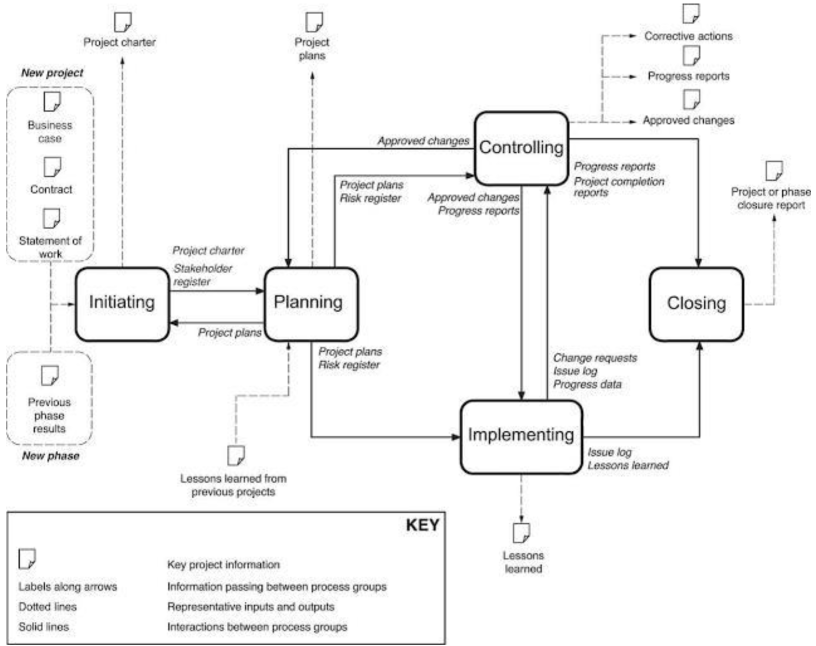
\includegraphics[width=\linewidth]{key_project_process_groups.png}
\end{figure}


\colorbox{green}{\textbf{Stakeholders}} - The entities involved with a project

Key \colorbox{cyan}{Elements} of a project;\\
\bulletPoint Business case - the justification of the project\\
\bulletPoint Plan\\
\bulletPoint Resources\\
\bulletPoint Scope\\
\bulletPoint Governance Structure - stakeholders, project team, project manager\\
Includes the boundaries of decision making for each role involved\\
\bulletPoint Budget/Costs\\
\bulletPoint Project methodology

\newpage

Project \colorbox{cyan}{Variables} aka “Project Triangle” or “Triple” or “Quadruple” Constraint:
\begin{figure}[h!]
  \centering
  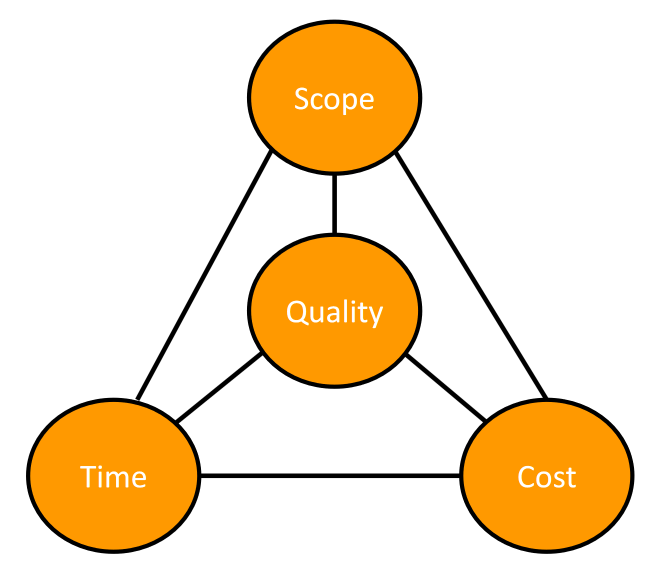
\includegraphics[width=20em]{project_variables_triangle.png}
\end{figure}

The time (schedule) of projects and their cost are interrelated, assuming that
the quality expectations have been defined and remain unchanged

\textbf{Main \colorbox{cyan}{distinguishing characteristics} of IT Projects}, in comparison with projects in other domains:\\
\bulletPoint The end-product is \colorbox{yellow}{intangible}\\
The end-product (e.g. software) is harder to be seen (“touched”). IT Project
Managers and other stakeholders \colorbox{pink}{cannot see progress} by simply looking at the
artefact that is being constructed. Take, for e.g., a web page with no back-end,
you may assume that it is done and ready to be shipped.\\
\bulletPoint Degree of \colorbox{yellow}{Uniqueness}\\
Most software projects are usually \colorbox{pink}{different} in a number of ways from previous
projects. Even managers who have significant experience may find it \colorbox{pink}{difficult to
  anticipate issues}. IT Systems are extremely \colorbox{pink}{human-intensive} and humans are
\colorbox{pink}{non-linear} systems! Even if a single individual is changed between two of the
same project, it can make a big difference\\
\bulletPoint Degree of \colorbox{yellow}{Uncertainty/Change}\\
\colorbox{yellow}{Requirements} of most IT projects \colorbox{yellow}{change} during the project due to a number of
reasons (e.g. business needs, market changes)\\
\bulletPoint Degree of \colorbox{yellow}{inter-dependencies}\\
IT Systems \colorbox{pink}{rarely live in isolation} and there exists a significant degree of
interdependencies to other systems/overall IT environment. A change or defect
may trigger a \colorbox{pink}{cascade of effects}.\\
\bulletPoint Communication / Common \colorbox{yellow}{Terminology}\\
There is often a \colorbox{yellow}{lack of a common vocabulary} between IT and Business people,
and even between IT people, mainly due to the proliferation of terms, lack of
standardization, the pace of technology evolution, inter-alia.\\

\chapter{Project Pre-Initiation}

\section{The business case}
"To \colorbox{yellow}{document the justification} for the undertaking of a project based on
the \colorbox{yellow}{estimated cost} of development and implementation against the \colorbox{yellow}{risks}
and the anticipated \colorbox{yellow}{business benefits} and savings to be gained. The total
business change must be considered, which may be much wider than just
the project development cost." (Prince2).

Determine that the estimated effort and time \colorbox{pink}{will be worth} the expenditure.

The document can be, for e.g., a PowerPoint

The \colorbox{yellow}{ongoing viability} of the project against the Business Case should be
\colorbox{yellow}{monitored} during the project.

\textbf{Typical \colorbox{cyan}{Elements} of a Business Case}:\\
\bulletPoint Problem statement and project \colorbox{yellow}{objectives}\\
\bulletPoint Summary of \colorbox{yellow}{scope} and any alternatives/options\\
\bulletPoint \colorbox{yellow}{Costs and Investment} Appraisal\\
\bulletPoint \colorbox{yellow}{Benefits} expected (quantitative, i.e. expressed in measurable terms against today’s\\
situation, and qualitative)\\
\bulletPoint \colorbox{yellow}{Risks} (summary of the key risks of the project)\\
\bulletPoint Timescales (summary of \colorbox{yellow}{plan})\\
\bulletPoint \colorbox{yellow}{Assumptions/Constraints}

Rule of Thumb: Should tell a “compelling story”, supported by facts/evidence!

\section{Investment Appraisal}

\subsection{CAPEX \& OPEX}

\textbf{Capital expenditures (\colorbox{green}{CAPEX})} is \colorbox{yellow}{funds} (money) \colorbox{yellow}{spent} in order to \colorbox{yellow}{create future benefits} for an organization, i.e.
purchasing new fixed assets (e.g. equipment, property, buildings) or extending the value (useful life) of existing assets
beyond the taxable year.

\textbf{An Operating Expense (\colorbox{green}{OPEX})} is any \colorbox{yellow}{on-going cost} for \colorbox{yellow}{running} (operating) the business (e.g. property rent, office
stationary, utility bills, travel expenses, personnel salaries).

For example, the purchase of a printer is a CAPEX cost whereas the annual expenses for paper, toner, power and the
maintenance of the printer are OPEX costs.

Other common OPEX examples are the cost of personnel and facility
expenses (e.g. rent, electricity).

\newpage

For accounting/tax purposes, capital expenditures must be amortized/\colorbox{pink}{depreciated} over
the span of several years. We \colorbox{pink}{must define a 'useful lifetime'}.

Example: the straight-line depreciation of a computer over 4 years, if it was purchased at a cost
of £1000 and will have a salvage value of £400, is £150 per year ((1000 — 400)/ 4 years)

\subsection{TCO}

\textbf{Total Cost of Ownership (TCO)}\\
In business decision-making it is important to be able to determine the costs (direct and indirect) of
assets and/or to have a cost basis for establishing the total (financial) value of an investment.

A common means used for that purpose is called the Total Cost of Ownership (TCO), i.e. a financial
\colorbox{yellow}{estimate} whose puprose is to determine the cost of \colorbox{yellow}{acquiring and maintaining} (operating) an asset
(e.g. a product or IT system) \colorbox{yellow}{over a number of years}.

E.g., the TCO of a car is the cost of the car + everything else you will need for it,
like insurance, gas, parking spaces, etc.

The cost of operation is \colorbox{pink}{normally for 5 years}, 10 years if it is a larger system

\begin{figure}[h!]
  \centering
  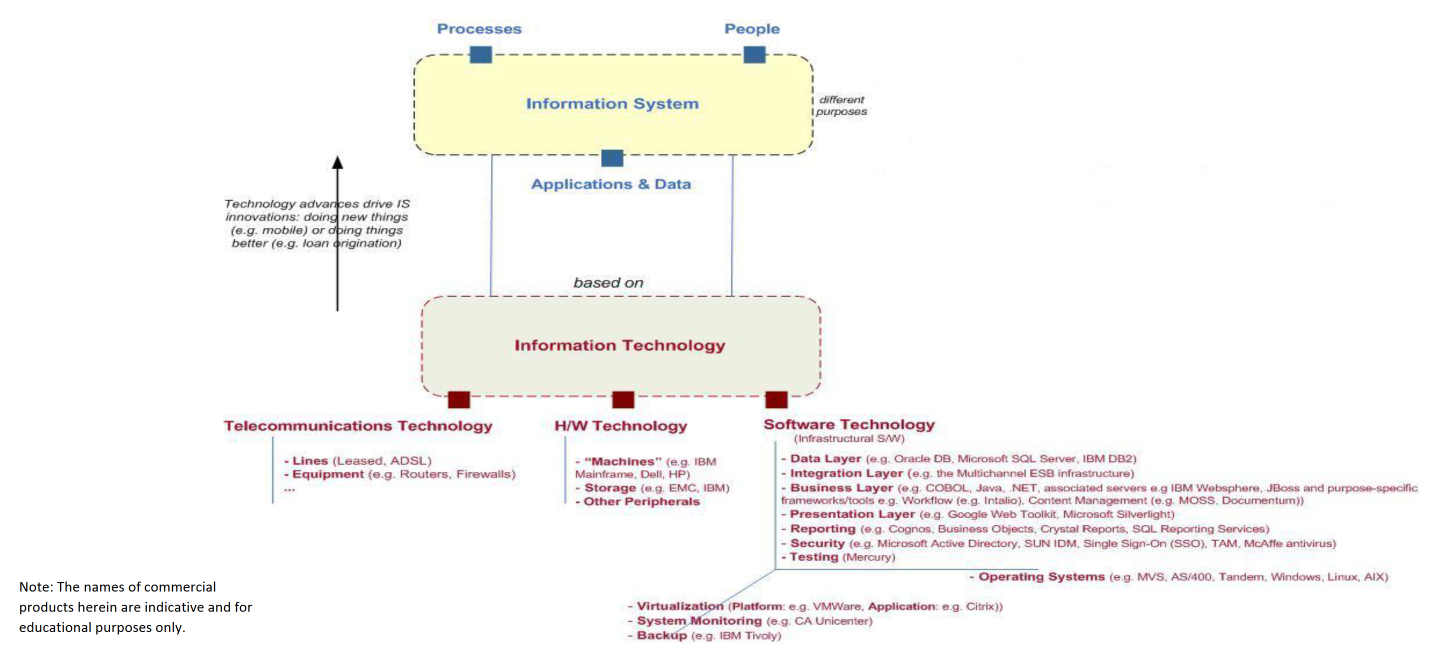
\includegraphics[width=\linewidth]{TCO.png}
\end{figure}

(dashes (-) in red are costs that are a part of the TCO for a system)

The \colorbox{yellow}{users} of some software \colorbox{yellow}{see} something that is generally called the '\colorbox{green}{Information system}'.
The user is \colorbox{yellow}{doing some task}, and the \colorbox{yellow}{system supports this task}, e.g., ticket booking on a website.

Information Technology is a world of stuff that is used to create and operate
what the end user sees.

\newpage

\colorbox{cyan}{Main Acquisition} Cost (CAPEX) \colorbox{cyan}{elements}:\\
\bulletPoint \colorbox{yellow}{S/W licenses}\\
i. Application SW licenses\\
ii. Software Technology related licenses\\
\bulletPoint \colorbox{yellow}{H/W} Technology (e.g. servers, storage, workstations, appliances)\\
\bulletPoint \colorbox{yellow}{Telecommunications} Technology and Lines\\
\bulletPoint Acquisition \colorbox{yellow}{research}/decision/procurement costs\\
\bulletPoint Implementation/\colorbox{yellow}{Installation} Services\\
\bulletPoint \colorbox{yellow}{Development} and Customization Services\\
\bulletPoint \colorbox{yellow}{Integration} Services\\
\bulletPoint \colorbox{yellow}{Testing}\\
\bulletPoint \colorbox{yellow}{Consulting}\\
\bulletPoint \colorbox{yellow}{Training}\\
\bulletPoint \colorbox{yellow}{Travel}

\colorbox{cyan}{Main Operation} Cost (OPEX) \colorbox{cyan}{elements}:\\
\bulletPoint \colorbox{yellow}{S/W maintenance}\\
i. Application SW\\
ii. Software Technology related\\
iii. Development/Customizations maintenance\\
e.g., Redhat maintenance, version updates, etc.\\
\bulletPoint \colorbox{yellow}{H/W} Technology \colorbox{yellow}{maintenance}\\
Usually around 10\% of the acquisition fee\\
\bulletPoint \colorbox{yellow}{Telecommunications} Technology and Lines\\
\bulletPoint \colorbox{yellow}{Recurring} Data Center \colorbox{yellow}{Costs}, e.g. floorspace, electricity\\
\bulletPoint \colorbox{yellow}{Recurring Operations} Costs e.g. backups, patches.\\
\bulletPoint \colorbox{yellow}{Training}

\colorbox{pink}{Some costs should be considered \textbf{per} target environment},\\ i.e. Live/Production,
Disaster, Testing, Development

\textbf{Full time equivalent (\colorbox{green}{FTE})} - the \colorbox{yellow}{time it takes} a defined \colorbox{yellow}{number of people}
to \colorbox{yellow}{work on a} \colorbox{yellow}{task full-time}

\subsection{Return on Investment (ROI)}
When applied to projects, \colorbox{green}{ROI} is a measure (a calculation/estimate) of the \colorbox{yellow}{value of a project}

the \colorbox{yellow}{benefits} received from the project \colorbox{yellow}{against the total costs} of the project
\colorbox{yellow}{over a timeframe} so that to know the value of an investment before spending time
and money on it.

ROI is \colorbox{pink}{usually expressed as a number} (percentage) \colorbox{pink}{on an annual basis}. For example, in its simple form,
£100,000 is invested and it earns £120,000, annually. This gives a ROI of 20\%.

Note that this is an \colorbox{yellow}{average} number and if the investment spans several years it
\colorbox{pink}{ignores the} \colorbox{pink}{\textbf{“time value of money”}}, i.e. the fact that the current value
of an amount of money differs to the value of the same amount of money in the future
(The more in the future you go, the less the same amount of money today has as value).

\subsection{Payback Period (PP)}
The \colorbox{yellow}{length of time} taken to \colorbox{yellow}{repay the initial \textbf{capital} cost}

i.e. “in what timeframe does a project pay for itself”?

Note that the PP method \colorbox{pink}{does not take into account the time value of money}.

\subsection{Net Present Value (NPV) / Discounted Cash Flows Valuation}

“\colorbox{yellow}{How much} does this investment \colorbox{yellow}{worth in today’s money}?”
— \colorbox{pink}{takes into account the time} \colorbox{pink}{value of money}.

Allows evaluating an investment by valuing at the same point in time, i.e. the present, the cash payments and
cash receipts expected to be made over the lifetime of the investment.

\textbf{Future Value}: the \colorbox{yellow}{value at a future date} of an amount invested today.\\
$Future Value = AmountInvested * (1 + InterestRate)^N$ ,\\ where $N$ is the number of periods we are measuring in the future

\textbf{Present Value}: the \colorbox{yellow}{value today} of a \colorbox{yellow}{payment that is promised} in the future (or else how much should be
invested today in order to realize the future value)\\
$Present Value = FutureAmount / (1 + InterestRate)^N$

The \colorbox{pink}{higher the interest rate, the lower the present value}. Therefore, the \colorbox{yellow}{interest rate} in the present value
calculation is called the \colorbox{green}{discount rate}. The further in the future, the lower the present value.

\textbf{Discount rate}: $1 / (1 + InterestRate)^N$

\textbf{Net Present Value (\colorbox{green}{NPV})}: is the \colorbox{yellow}{sum of the present values} (PV) \colorbox{yellow}{of all Net Cash Flows} \colorbox{yellow}{during the
  period} into consideration for the investment

\colorbox{green}{Net Cash Flows} are the \colorbox{yellow}{Inflows minus Outflows} where: inflows are the funds received and
outflows are the funds paid out.

NPV is the \colorbox{yellow}{sum of all} terms $A_t / (1 + r)^t$ , where,\\
\bulletPoint $t$: the time of the cash flow,\\
\bulletPoint $r$: the discount rate\\
\bulletPoint $A_t$ :the net cash flow (inflow minus outflow) at time $t$

$$NPV = \sum_{t=0....n} A_t / (1 + r)^t$$

NPV \colorbox{pink}{can be used} as a basis for \textbf{\colorbox{pink}{comparison} across investments} (i.e., will I invest in projectA or projectB) and bringing everything in \colorbox{pink}{today's terms}.

\newpage

\begin{figure}[h!]
  \centering
  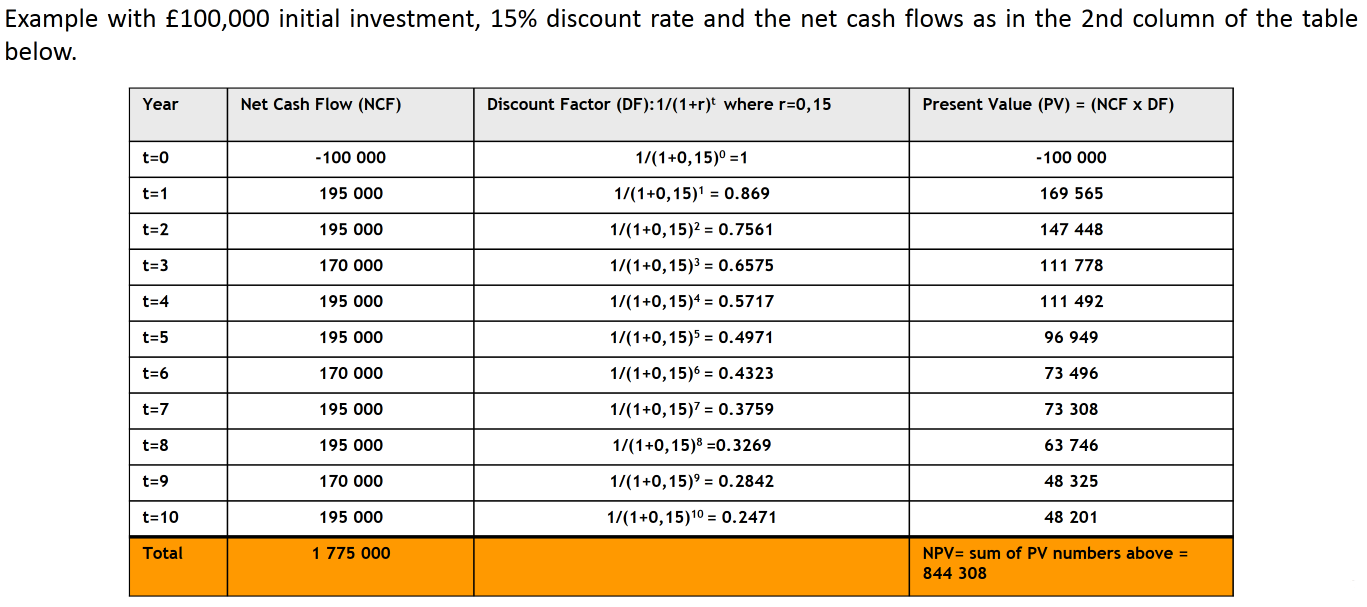
\includegraphics[width=\linewidth]{npv_example.png}
\end{figure}

So if we are estimating here that we will get £1,775,000 after 10 years,
we will actually be getting £844,308 (since that is what that amount is worth,
10 years in the future)

\subsection{Project Cost Estimation and Budgeting}
\colorbox{cyan}{Types of cost estimates}:
\begin{figure}[h!]
  \centering
  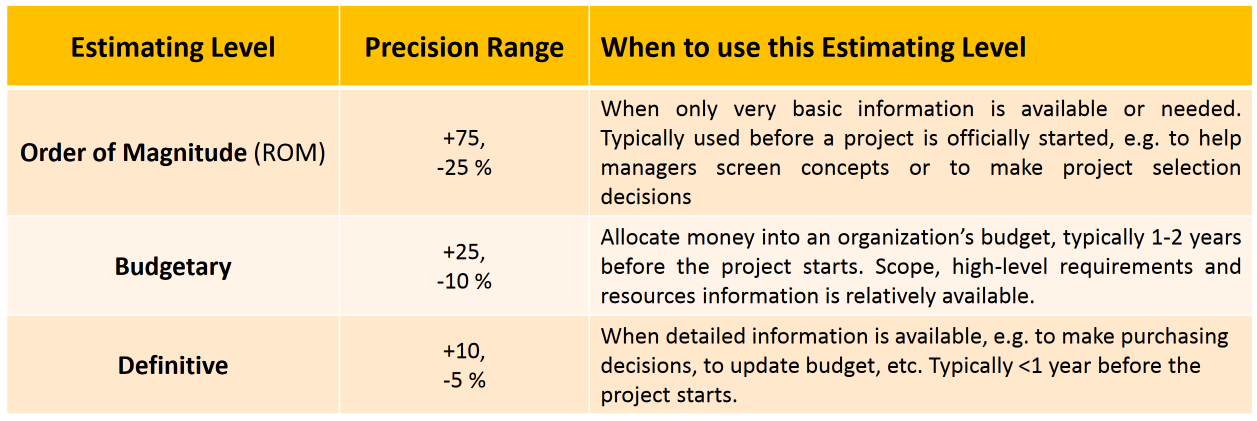
\includegraphics[width=\linewidth]{types_of_cost_estimates.png}
\end{figure}

ROM is \colorbox{pink}{Rough} order of magnitude, \colorbox{pink}{you know little detail}, for e.g., an e-commerce site (and that's it)

\colorbox{pink}{Budgetary} is more precise, you have more detail about what the project involves,
and it \colorbox{pink}{tends to become the} \colorbox{green}{baseline} \colorbox{pink}{budget} - the budget a project \colorbox{yellow}{starts with}.

\newpage

Main \colorbox{cyan}{estimation approaches}:
\begin{figure}[h!]
  \centering
  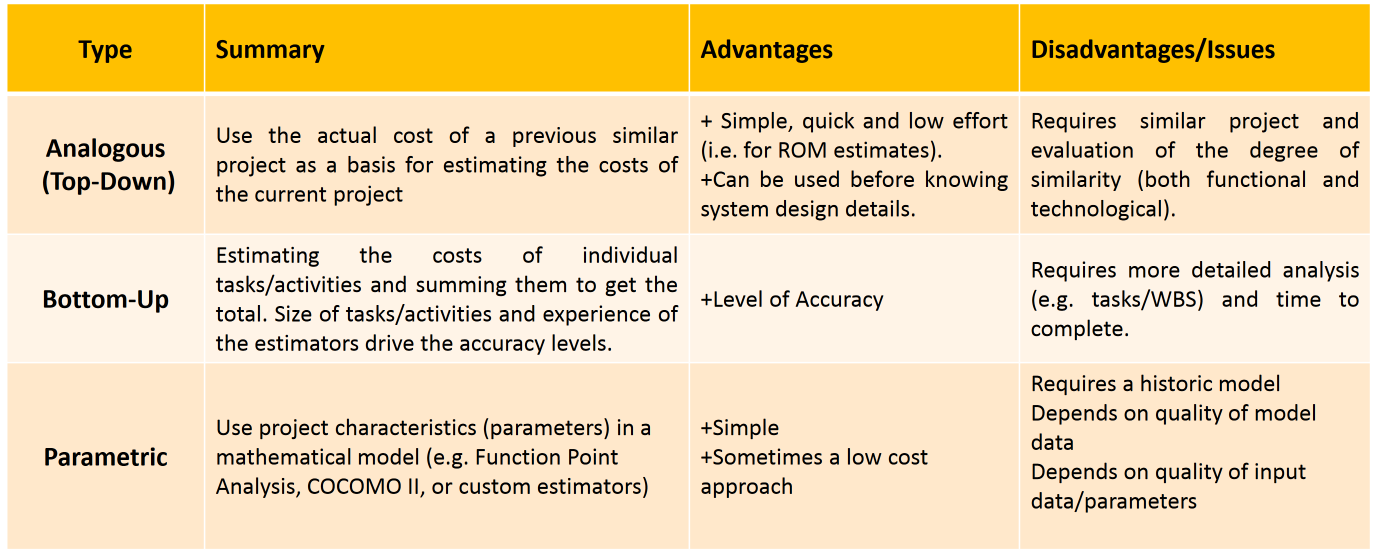
\includegraphics[width=\linewidth]{cost_estimation_approaches.png}
\end{figure}

Additional Approaches:\\
\bulletPoint \textbf{Delphi Method / Wideband Delphi}: seek \colorbox{yellow}{Expert Advice}, usually from a number of experts
\colorbox{yellow}{until they agree} on a common estimate.\\
\bulletPoint \textbf{Three-point Estimate}: \colorbox{yellow}{estimate} the Most Probable (MP), Optimistic (O) and Pessimistic (P) cost
for an item. Next use a weighted formula, e.g. the \colorbox{yellow}{PERT formula},\\
$E = (4 * MP + O + P) / 6$

\colorbox{pink}{Estimation of software development is the most difficult task} since everything else has set prices (hosting, hardware, etc.)

\subsubsection{Important Rules of Thumb / Checklist}
\begin{enumerate}
  \item In your estimation deliverable, explicitly state the underlying \textbf{Scope / Details} and any applicable \textbf{Assumptions} and \textbf{Rationale}.
  \item \textbf{Be honest!}
  \item \textbf{Do not do it alone}, i.e. do not tell people how long it will take them to do their work! Gain team and subcontractors
        consensus before you deliver your estimate.
  \item \textbf{Use historical information}, but adjust accordingly. Hence, \textbf{keep quality cost records of past projects!}
  \item Use a \textbf{combination} of \textbf{both methods} and \textbf{people} to estimate.
  \item Distinguish \textbf{Effort Vs Duration} (FTEs Vs Calendar days). In the latter, do not forget holidays!
  \item Be aware of the \textbf{organizational rules on effort/costs} (e.g. taxes (VAT), labour unit costs, mdays/hours, working days)
  \item Be aware of the \textbf{organizational rules on controls/required deliverables}, e.g. security checks, legal checks, preparation of
        manuals, training. These will imply additional tasks/effort.
  \item Adjust estimates for \textbf{loading factors} (e.g. multiple groups involved, remote locations, traveling, culture/language barriers)
  \item Include \textbf{reasonable Reserves} (for unanticipated/changing circumstances). Unreasonable reserves have impact (why?)
  \item Do not forget effort to: (i) gather detailed, agreed requirements, (ii) test (all types of testing), (iii) setup system in different
        environments (and have test data available), (iv) number and complexity of interfaces to other systems.
  \item \textbf{Human beings are biased towards underestimation}. Do not be too optimistic based on your own abilities. We also have anchoring
        bias - we \textbf{rely too heavily on the first piece of information we recieve}. This effects both the first estimate (wrong estimate from
        an expert sticks, and you ignore others) and when estimates go wrong (you tell your manager you need an extra 5 days but
        they still see it as being done in the original time-frame).
  \item If \textbf{imposed with infeasible deadlines and budget from management, do not merely accept! Negotiate focusing on the
          equilibrium of scope/time/quality/cost (rather than cost alone)!} Moreover, be cautious on initial estimates as management
        never forget these, but rarely remember subsequent changes/adjustments. Keep them informed formally and keep records.
        \textbf{Be prepared to be challenged on your estimates, hence make sure they are defensible!}
\end{enumerate}

\subsubsection{Project Budget}

The \colorbox{yellow}{process and relevant artifact} of \colorbox{yellow}{allocating the estimated} costs, labor and
material, over time.

The \colorbox{pink}{main goal} is to \colorbox{pink}{establish an authorized cost baseline} and the key benefit
is that it determines the cost baseline \colorbox{pink}{against which} project performance can be \colorbox{pink}{monitored} and
controlled.

It also facilitates the organization’s overall costs and cash flow management.

Budget is \colorbox{pink}{usually split monthly}

The project manager is \colorbox{pink}{not in charge} of the budget, they must make sure they
do not exceed the budget, ask for approvals, and formally communicate how they
stand with the budget

\bulletPoint \colorbox{yellow}{Detailed} Budget \colorbox{yellow}{preparation} is typically \colorbox{yellow}{part of} the Project \colorbox{yellow}{Planning process} rather than the
Pre-Initiation phase. However, in practice, it is common that a project allocated budget exists at
this stage (the measure is reliable)  (e.g. with a high-level allocation in time)

\bulletPoint Apart from the cost estimates, the budgeting process has a number of inputs which will be
discussed later (e.g. WBS, project plan/schedule, actual project team, risks).

\bulletPoint It also \colorbox{pink}{typically includes Reserves} (Contingency and Management Reserves)\\
\colorbox{green}{Contingency Reserves} - for \colorbox{yellow}{identified risks} that have \colorbox{yellow}{planned} potential actions\\
\colorbox{green}{Management Reserves} - for things we \colorbox{yellow}{can't anticipate} in the project

\bulletPoint Most \colorbox{pink}{organizations have their own process} and rules on how to prepare project budgets (e.g.
on the way to include FTE costs, on depreciation, on taxation, on currency).

\bulletPoint Budgets have \colorbox{yellow}{deviations}, which \colorbox{yellow}{should be managed} (as part of what is known as Project Cost
Management), and therefore could change over the course of the project – such changes
should be \colorbox{yellow}{formally approved and communicated}.

\newpage

\subsection{IT Systems Acquisition Models}

\colorbox{cyan}{Models to acquire a system}:\\
\bulletPoint \colorbox{green}{Custom-built} - \colorbox{yellow}{In-house or Outsourced} / \colorbox{green}{Offshored} (the company outsourced to is in a different country)\\
\bulletPoint \colorbox{green}{Package-based} (\colorbox{yellow}{ready-made} software that more or less satisfies our needs) - \colorbox{green}{Commercial} (\colorbox{yellow}{Pay a license} to the vendor) or \colorbox{green}{Open Source} (typically don't pay a license but may pay annual maintenance or support) - Any \colorbox{pink}{customizations needed will be custom-built}\\
\bulletPoint \colorbox{green}{SaaS} - Cloud - Like package based, \colorbox{yellow}{paying} for the system \colorbox{yellow}{as a whole}, but we do not download it, instead we use a \colorbox{yellow}{cloud provider} to \colorbox{yellow}{run the system for us}, on their servers \\
\bulletPoint PaaS - Cloud\\
\bulletPoint IaaS - Cloud\\

\subsubsection{Custom-Built}
software/system that is \colorbox{yellow}{constructed} (from “scratch”) \colorbox{yellow}{according} to an
\colorbox{yellow}{organization requirements} / specifications.

Two main sourcing variations:\\
\bulletPoint In-house\\
\bulletPoint Outsourced/Offshored

Main \colorbox{cyan}{Advantages}:\\
\bulletPoint \colorbox{yellow}{Flexibility}\\the software can be constucted/modified according to the specific business needs\\
\bulletPoint \colorbox{yellow}{Control}\\the organization has limited dependency on 3rd parties (only partially on the outsourcing case - intellectual property still belongs to us)\\
\bulletPoint Easier \colorbox{yellow}{integration} with (our) other systems \\
\bulletPoint No \colorbox{yellow}{license fees or maintenance fees} (maintenance - this may not be the case on the outsourcing scenario)

Main \colorbox{cyan}{Issues}:\\
\bulletPoint  Project risk and cost\\the \colorbox{yellow}{organization should assume the risks and costs} of the project (\colorbox{yellow}{including the quality} of the result)\\
\bulletPoint  \colorbox{yellow}{Less-time-to-market} (more time needed to develop the software)\\
\bulletPoint  \colorbox{yellow}{Miss opportunity} to obtain business know-how/adopt \colorbox{yellow}{Best Practices} (which are typically embedded in packaged software applications)

\subsubsection{Package-based}
Also known as “off-the-shelf” software. A ready-made software that implements a certain
business functionality, for example, ERP and CRM.

A packaged (ready made) software can be divided into two categories: commercial and open source.

A commercial packaged software is built in order to be sold, i.e. is only available to an organisation that
has agreed to pay a certain fee for it, typically\\
(i) License fee (per number of package users or based on number of CPU’s used on the servers that the
package is installed)\\
(ii) Annual Maintenance fee (for correction of errors and right to use the future versions of the package
without licensing).

Its \colorbox{pink}{source code} is \colorbox{pink}{typically not made available} to the public.\\
Open source is software whose source code is available to the public to use and change. Typically
created in a collaborative way and improvements made are shared by the community.

\colorbox{pink}{Common misconception: Open Source software is always free} of charge – this may not be the case!.  Different
open source licenses exist, particularly for profit-organizations to have the right to use open source.

Moreover, for organizations adopting open source a typical case is to pay annual support fees to a
vendor supporting the software (e.g. Red Had, JBoss) – what is known as commercially supported open
source.

Support is an OPEX cost whereas a license is a CAPEX cost

If a \colorbox{pink}{package meets more-or-less 85\% of your needs}, it is
\colorbox{pink}{best to go with the package}\\ \colorbox{pink}{(or less than 50\% is
  customizations)} since customizations take time and a vendor may update
the out-of-box software within that time-frame

For Commercial Package-based software:

Main \colorbox{cyan}{Advantages}:\\
\bulletPoint Faster \colorbox{yellow}{time-to-market} (project implementation)\\
\bulletPoint Opportunity to obtain business know how/adopt \colorbox{yellow}{Best Practices} (which are typically embedded in packaged software applications)

Main \colorbox{cyan}{Issues}:\\
\bulletPoint Less \colorbox{yellow}{flexibility} (if the package needs to be modified (customized) to meet specific organizational needs – such customizations require extra fee and may lead to cost increase)\\
\bulletPoint \colorbox{yellow}{Control} — the organization has dependency on 3rd parties (the package vendor)\\
\bulletPoint License/maintenance/support \colorbox{yellow}{fees}\\
\bulletPoint \colorbox{yellow}{Integration} to other system may be more difficult (particularly if the package has not integration capabilities embedded)

For Open Source (Vs Commercial) Package-based software:

Main \colorbox{cyan}{Advantages}:\\
\bulletPoint Less \colorbox{yellow}{cost} (or at least less CAPEX (investment) cost - but this may not be
the case for OPEX (annual) cost)\\
\bulletPoint Availability of \colorbox{yellow}{source code}

Main \colorbox{cyan}{Issues}:\\
\bulletPoint \colorbox{yellow}{Support} issues — potential difficulties to get support
or feedback on the open source software. \\
\bulletPoint \colorbox{yellow}{Maturity} in the functionality provided\\
\bulletPoint \colorbox{yellow}{Scalability} (particularly for large installations)\\
\bulletPoint \colorbox{yellow}{Legal/IP Issues}

\newpage

\subsubsection{Cloud}
“computer \colorbox{yellow}{users} (end users and organizations) \colorbox{yellow}{conveniently rent access} to fully featured
applications, to software development and deployment environments, and to computing infrastructure
assets such as network-accessible data storage and processing.”

\begin{figure}[h!]
  \centering
  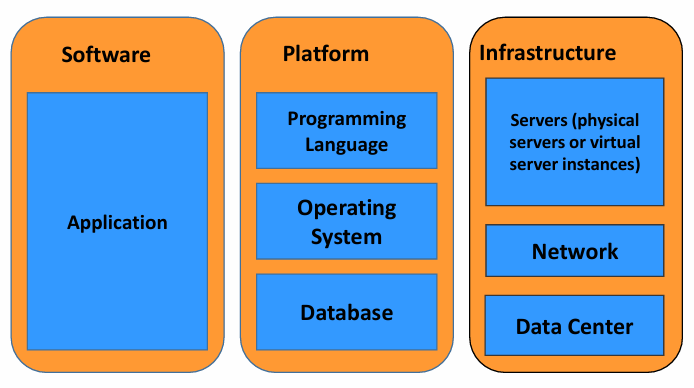
\includegraphics[width=\linewidth]{cloud_models.png}
\end{figure}

3 \colorbox{cyan}{main models}:\\
\bulletPoint Software as a Service (\colorbox{green}{SaaS}) - \colorbox{yellow}{cloud provider owns the app} and we \colorbox{yellow}{pay them to use} it\\
\bulletPoint Platform as a Service (\colorbox{green}{PaaS}) - we custom-build or buy a package and pay the cloud provider for a \colorbox{yellow}{platform to install it on}\\
\bulletPoint Infrastructure as a Service (\colorbox{green}{IaaS}) - we have all of the relevant software to run the app but we need \colorbox{yellow}{hardware from the cloud provider} to run it

Main \colorbox{cyan}{Advantages}:\\
\bulletPoint More \colorbox{yellow}{Flexible cost} model (less CAPEX, emphasis on OPEX )\\
\bulletPoint \colorbox{yellow}{Operational responsibility} to 3rd party (that typically has more expertise)\\
(Don't have to monitor its status, don't have to budget for upgrades or security patches, etc.)
\bulletPoint \colorbox{yellow}{Less in-house sourcing} requirements

Main \colorbox{cyan}{Issues}:\\
\bulletPoint Vendor Lock-in, Loss of \colorbox{yellow}{control}\\
\bulletPoint \colorbox{yellow}{Security} - at the mercy of the cloud provider\\
\bulletPoint \colorbox{yellow}{Integration}\\
\bulletPoint Build \colorbox{yellow}{expertise} in cloud optimized solutions and cloud related processes

\newpage

\subsection{Basics of Procurement and Contracts Management}
\colorbox{green}{Procurement}: the \colorbox{yellow}{process of acquiring products} or services from a 3rd party.\\
\colorbox{pink}{Often done via a (formal) bid (tender) process}.

\colorbox{cyan}{Key Documents}:-\\
Request For Information (\colorbox{green}{RFI})\\
Request for Quote (\colorbox{green}{RFQ})\\
Request for Proposal (\colorbox{green}{RFP})\\
An \colorbox{yellow}{invitation} for suppliers of a product or service to \colorbox{yellow}{submit a proposal} (as
part of a bidding process) in order to supply that product or service to
the entity that issued the RFP.

A company would \colorbox{pink}{usually research vendors} and \colorbox{pink}{choose} which companies to \colorbox{pink}{send the RFP} to

There is usually a \colorbox{pink}{scorecard} with some criteria for \colorbox{pink}{evaluating the proposals}. The proposals are evaluated by the 'Technical Evaluation Committee'.
The companies \colorbox{yellow}{also submit a financial} \colorbox{yellow}{proposal} separately

The RFP is a \colorbox{green}{formal document}; this means that \colorbox{yellow}{it can stand up in court} if someone claims that the process was not fair

The RFI and RFQ are \colorbox{pink}{a bit informal}. These \colorbox{pink}{help understand} if a company is \colorbox{pink}{capable}
\colorbox{pink}{of meeting} \colorbox{pink}{the requirements} before sending them the RFP. The RFQ also
helps secure a budget.

\colorbox{green}{Statement of Work}:\\
the \colorbox{yellow}{description of work required} for the procurement or as part of the contract.\\
A scope document with sufficient level of detail, clarity and non-ambiguity are
critical factors.

The SOW describes the \colorbox{yellow}{scope} of work, describing the capabilities of the
deliverable, what the end deliverable actually is (doesn't only need
to be software, e.g., manuals), the \colorbox{yellow}{schedule} of the
deliverables, \colorbox{yellow}{standards} that need to be followed,
how the organization will accept the deliverable, etc. e.g., location of
work (if they are providing people)

The SOW \colorbox{pink}{tends to be part of the contract} for the project.
\colorbox{pink}{Sometimes} a project \colorbox{pink}{can start} \colorbox{pink}{without the contract} as the contract takes
time to finalize with, for e.g., lawyers, and \colorbox{pink}{other documents are legally
  binding}. What you will definitely have is the software licensing partner
(The licensing is also a contract).

\newpage

Main \colorbox{cyan}{Types of Contracts}:

\colorbox{green}{Fixed Price} (Lump Sum)\\
\bulletPoint \colorbox{yellow}{Fixed scope} - risk - negotiations with the vendor\\
\bulletPoint \colorbox{yellow}{Fixed Total Cost} Vs Fixed Unit Price\\
\bulletPoint with / without incentive\\
\bulletPoint with \colorbox{yellow}{price adjustment}

\colorbox{green}{Cost-reimbursable} (aka Cost-Plus)\\
\colorbox{yellow}{Vendor agrees on the FTE}, the cost of the FTE and the profit on top of that cost (people are still payed for the real work time)\\
\bulletPoint Cost plus IncentiveFee (CPIF)\\
\bulletPoint Cost plus Fixed Fee (CPFF)\\
\bulletPoint Cost Plus Award Fee(CPAF)\\
\bulletPoint Cost Plus Percentage of Costs (CPPC)

Time and Material (T\&M)

\chapter{Project Initiation and (Initial) Planning}
Initiation tends to be a very critical stage, while being short in duration

\section{Project Stakeholders / Organization / Governance}
Stakeholder: Any party who is interested in, or affected by the outcome of the project.\\
e.g., departments, individuals, etc.

The Project governance structure:
\begin{figure}[h!]
  \centering
  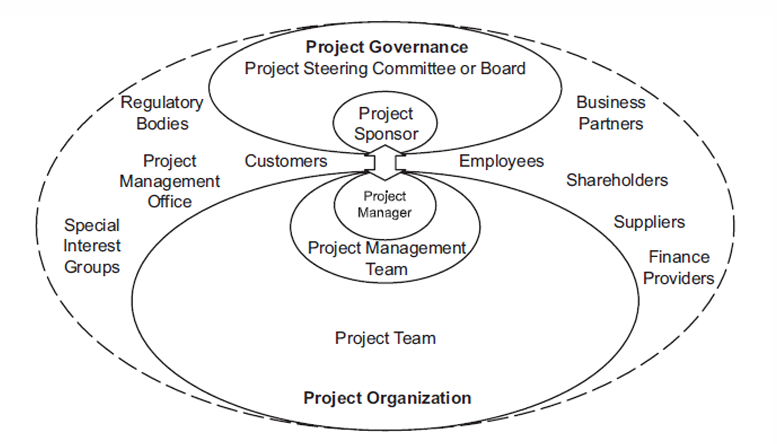
\includegraphics[width=\linewidth]{project_governance_structure.png}
\end{figure}

(Everyone not in an oval with a solid border is a stakeholder)

\subsection{Stakeholder analysis}
\bulletPoint Who gets the output?\\
\bulletPoint  Who provides the input?\\
\bulletPoint  Managers of input providers or output recipients\\
\bulletPoint  Who has related responsibilities?\\
\bulletPoint  Who gets the reward and benefits?\\
\bulletPoint  Who suffers the penalties and consequences?

Stakeholder analysis drives:\\
\bulletPoint Project organization/governance design\\
\bulletPoint Project process definition\\
\bulletPoint Communication planning\\
\bulletPoint Detailed requirements analysis\\
\bulletPoint Risk planning\\
\bulletPoint Testing and Training

To conduct a Stakeholder Analysis:\\
Goal: to increase their support throughout the project\\
\bulletPoint Identify all possible stakeholders and maintain a Stakeholder Register\\
\bulletPoint Determine who is an “Ally” and who is an “Adversary”\\
\bulletPoint Establish level of awareness, concern and interest\\
\bulletPoint Ask the Questions; Do they care?, Should they care?, Do we want them to care?\\
\bulletPoint Develop stakeholder assessment grid, e.g. a Power/Interest grid or a Power/Importance grid

\begin{figure}[h!]
  \centering
  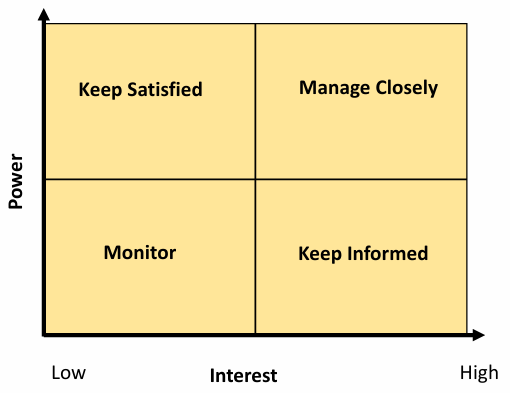
\includegraphics[width=.6\linewidth]{stakeholder_assessment_grid.png}
  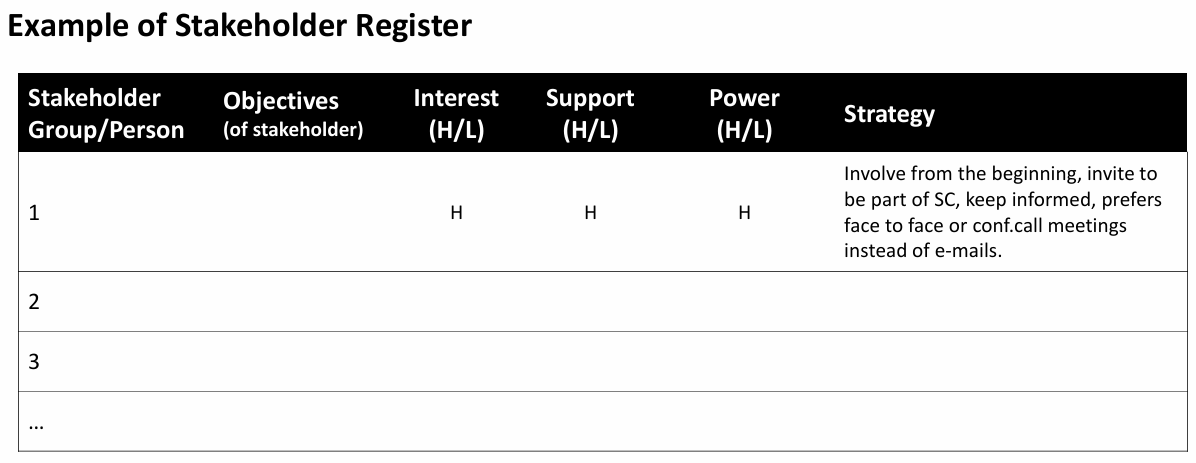
\includegraphics[width=\linewidth]{stakeholder_register.png}
\end{figure}

\subsection{The project governance structure}
Essentially, the project steering committee (decision makers - they steer the project)

Project Governance: the framework by which the project is directed and controlled, e.g.\\
i.   defining the team/management structure (including members' responsibilities),\\
ii.  policies/processed/methodologies to be used,\\
iii. limits of authority for decision-making,\\
iv.  stakeholders’ responsibilities/accountabilities,\\
v.   interactions such as reporting and the escalation of issues or risks.

\textbf{Key Roles:}\\
\bulletPoint The Project Sponsor (Executive):\\
authorizes and funds the project (via the Business Case), makes executives decisions
beyond the Project Manager’s authority, has the power to
overcome issues/conflicts/remove barriers (e.g., give more money) to project success (or cancel the project). They own the business case and the project, delegating it to the project manager.

\bulletPoint The Project Steering Committee or Board\\
provides senior (less than the sponsor) level guidance to the project and facilitates integration of the
PM team with functional units. Project Control and Assurance role. May
also act as Change Authority. Represents the key stakeholders of the project; provide guidance on important decisions that do not have to go to the sponsor.

\bulletPoint The Project Manager\\
leads projects activities and the day-to-day
management of the project. Responsible for project delivery.

\bulletPoint Project Management Team (aka Project Support)\\
supports the project manager (e.g. on administrative tasks).(Lots of bureaucracy)

\bulletPoint Project Team (Team Managers)\\
perform (coordinates) project activities.

\section{The Project Charter}

The Project Charter is a document that formally authorizes the Project and
assigns a Project Manager (and other roles). Typically includes the following
elements:\\
1. Objectives \& Business Case\\
2. High-Level Scope/Statement of work\\
3. High-level budget information\\
4. High-level timelines/target dates\\
5. Project organization/governance information.\\
6. Success criteria\\
7. Initial Set of Risks

In Prince2, a similar artefact pertains to what are known as the Project
Mandate and Project Brief documents which both provide input to what,
after planning, becomes a Project Initiation Document (PID) artefact.

Project Kick-Off Meeting takes place upon finalization of the Project Charter (The day the project officially starts - Everyone should be there; the project manager delivers a presentation so that everyone is aligned)

\section{Common Pitfalls and Best Practices}
\begin{figure}[h!]
  \centering
  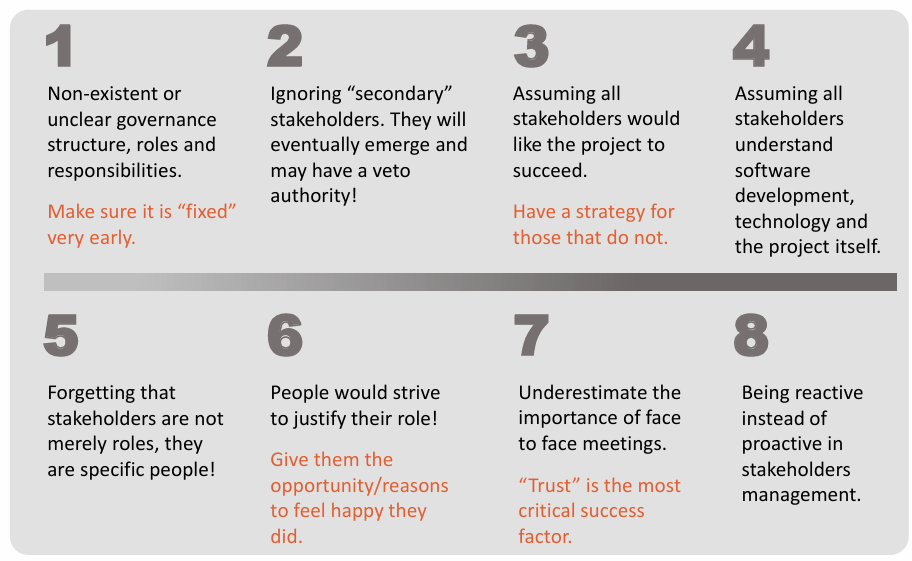
\includegraphics[width=\linewidth]{project_initiation_common_pitfalls.png}
\end{figure}


\chapter{The first/basic Project Planning Elements: Scope, Time, Resources, Communications.}

\section{Scope}

Scope Management Overview:

1. Define Scope Statement \& Requirements - know what you need to do\\
2. Create Work Breakdown Structure\\
3. Define Activities (produce an Activity List)\\

\subsection{Requirements}

Functional Vs non-Functional (process vs quality / HCI)\\
It's impossible for a system to meet all non-functional requirements - there will be trade-offs

A number of Issues:\\
\bulletPoint Stakeholders don’t know what they really want.\\
\bulletPoint Stakeholders express requirements in their own terms.\\
\bulletPoint Different stakeholders may have conflicting requirements.\\
\bulletPoint Organisational and political factors may influence the system requirements.\\
\bulletPoint The requirements change during the analysis process.\\New stakeholders may emerge and the business environment may change.\\
\bulletPoint Clarity and Unambiguity, Common Communication language, amalgamation (several different requirements may be expressed together)

Produce a document for requirements - can consist of use cases, user stories, etc.

Analysts try to map an interface between a customer and developer

\begin{figure}[h!]
  \centering
  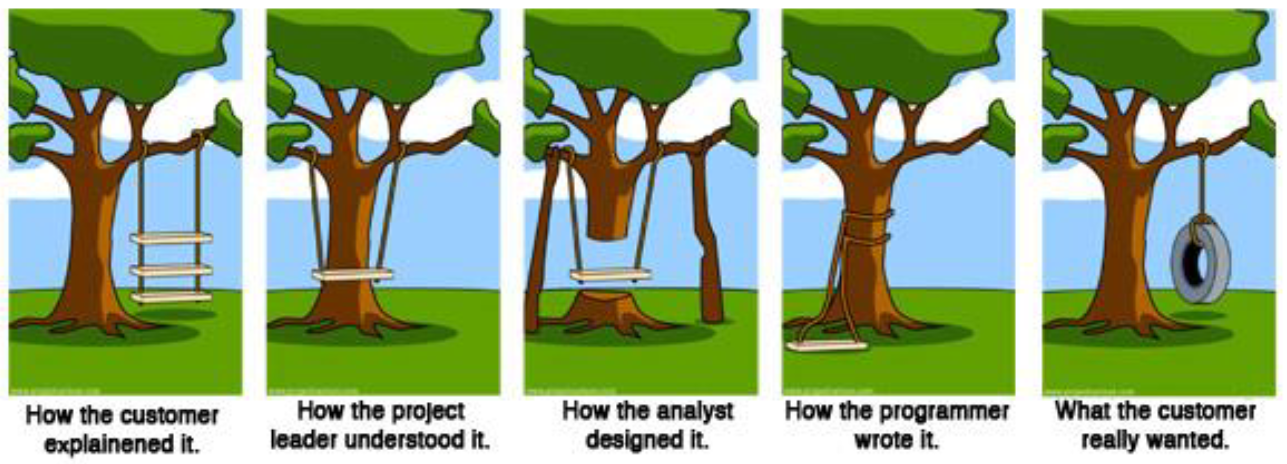
\includegraphics[width=\linewidth]{understanding_requirements.png}
\end{figure}

\newpage

\begin{figure}[h!]
  \centering
  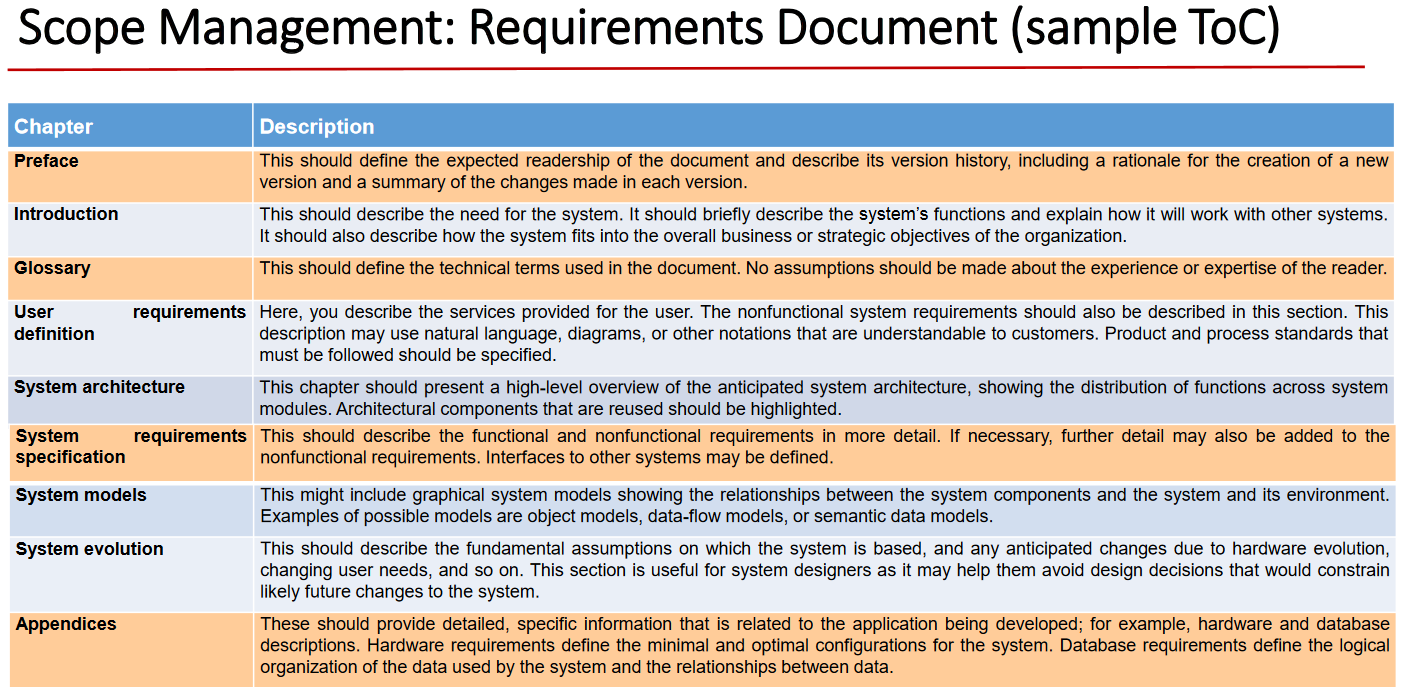
\includegraphics[width=\linewidth]{requirements_document.png}
\end{figure}

Context diagram to show high-level scope:

\begin{figure}[h!]
  \centering
  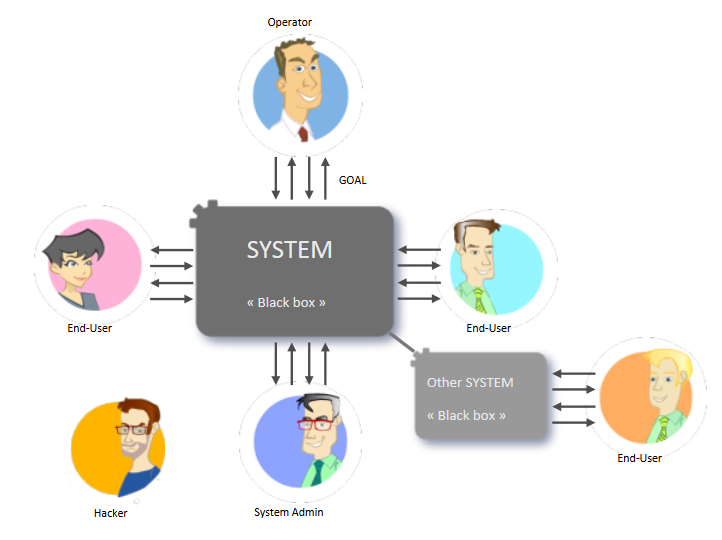
\includegraphics[width=35em]{scope_context_diagram.png}
\end{figure}

\newpage

Main Ways of Writing a Requirements Specification:

\bulletPoint Natural language:\\
The requirements are written using numbered sentences in natural language. Each sentence
should express one requirement.

\bulletPoint Structured natural language:\\
The requirements are written in natural language on a standard form or template. Each field
provides information about an aspect of the requirement.

\bulletPoint Graphical notations:\\
Graphical models, supplemented by text annotations, are used to define the functional
requirements for the system; UML use case and sequence diagrams are commonly used.

\bulletPoint Mathematical specifications:\\
These notations are based on mathematical concepts such as finite-state machines or sets.
Although these unambiguous specifications can reduce the ambiguity in a requirements
document, most customers don’t understand a formal specification. They are also time-
consuming. Used mostly in safety-critical systems

Some Methods of Requirements Elicitation:

\bulletPoint Interviews\\
\bulletPoint Brainstorming workshops - normally used when there are no mature ideas\\
\bulletPoint Questionnaires and Surveys\\
\bulletPoint Ethnography - observe stakeholders in their working environments\\
\bulletPoint Use Case Analysis, User Stories\\
\bulletPoint Prototypes/Modelling\\
\bulletPoint Demonstrations of current operating environment\\
\bulletPoint 5-Why Analysis - keep asking WHY\\
\bulletPoint Fishbone diagrams\\
\bulletPoint Use experience / examples / blueprints from previous projects

\subsection{Work Breakdown Structure (WBS)}

WBS is a “deliverable-oriented grouping of the work involved in a project that defines its total
scope” (PMBoK).

Can be a hierarchy of deliverables or activities/tasks/work items. The goal is to
decompose what needs to be done (task) in a project into smaller chunks.

Teams may organize the WBS around\\
i. project products or\\
ii. project phases or\\
iii. project management process groups.

In “traditional” PM, WBS is very important as it provides the basis for project schedule, costs,
resources planning and change management.

WBS typically have an accompanying WBS Dictionary – a document that describes/provides
details on each of the elements of the WBS (e.g. a more detailed description, start-end dates,
quality criteria/requirements, required resources, applicable technical content, applicable costs)

\newpage

For example, a product breakdown structure (a specialization of the work breakdown structure):
\begin{figure}[h!]
  \centering
  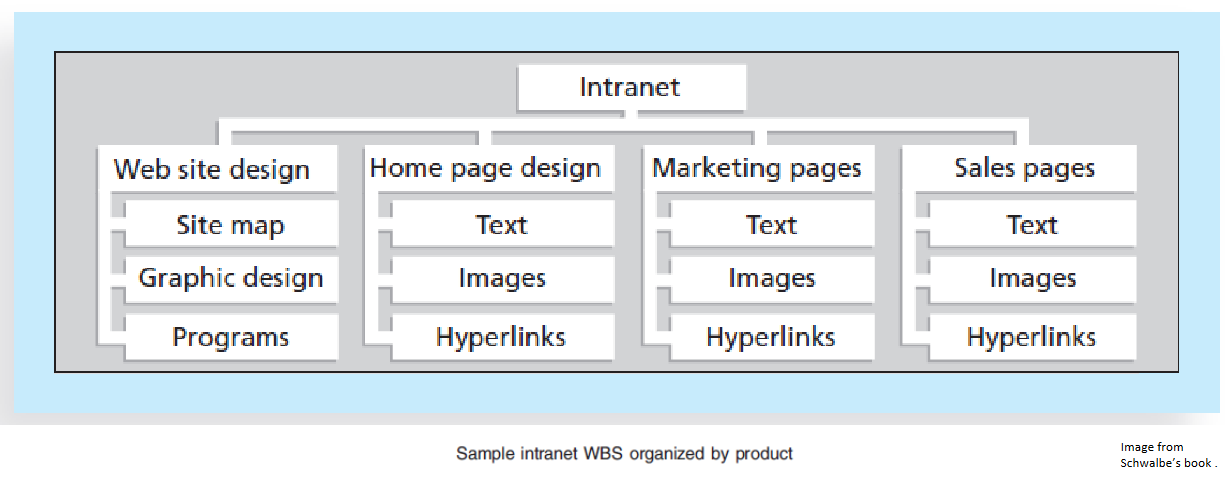
\includegraphics[width=\linewidth]{product_breakdown_structure.png}
\end{figure}

Another example, a task based breakdown:
\begin{figure}[h!]
  \centering
  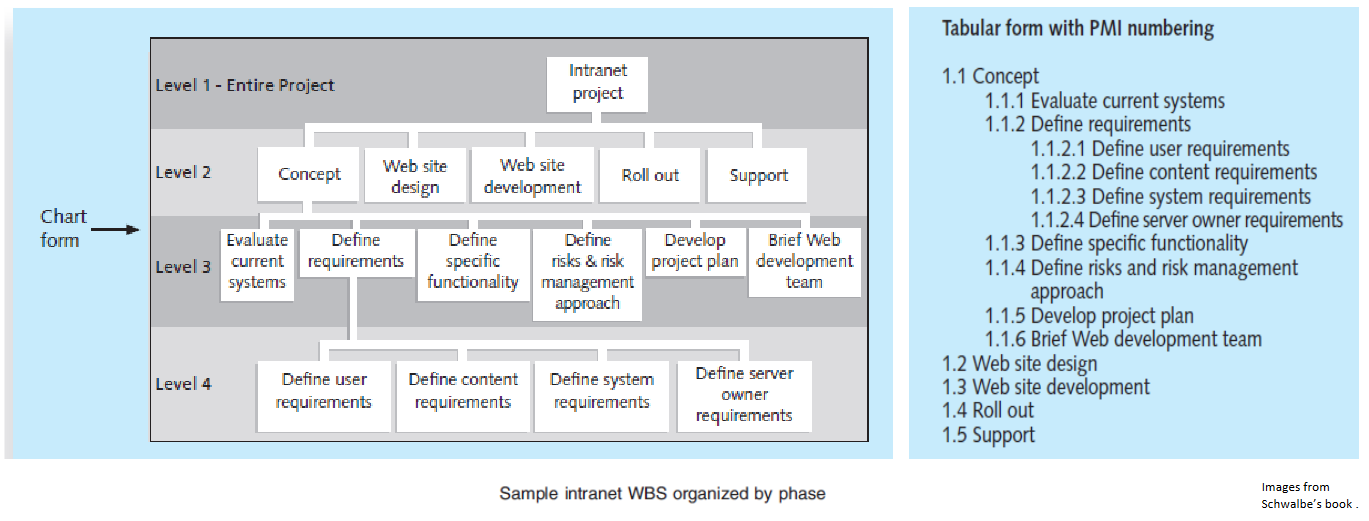
\includegraphics[width=\linewidth]{task_based_breakdown.png}
\end{figure}

In Prince2, the concept of Product Breakdown Structure (PBS) is explicitly used.

PBS is defined as “a hierarchical structure that breaks down a final product into its
constituent sub-products”. The sub-products include any Prince2 management artefacts to
be produced.

The PBS is usually accompanied by a Product Flow Diagram (PFD) that defines the
sequence in which the products will be developed.

Methodology to organize and split work: IBM’s MITP methodology for WPS:

Level 1. Project\\
Level 2. Deliverables (e.g. SW, HW, Manuals, Training)\\
Level 3. Components to produce deliverables (e.g. modules but also items such as tests)\\
Level 4. Work-Packages, i.e. major work items or collections of related tasks required to
produce a component\\
Level 5. Fine-grained Tasks (single person responsibility)

\newpage

\begin{figure}[h!]
  \centering
  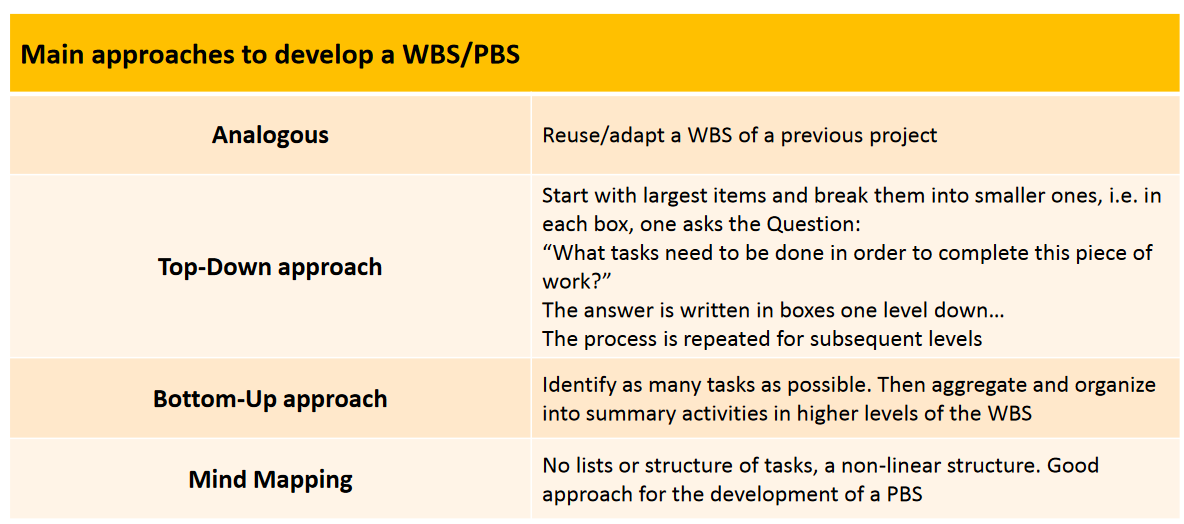
\includegraphics[width=\linewidth]{approaches_to_WBS.png}
\end{figure}

\section{Time}

Scheduling Management Steps/Overview:\\
1. Sequence Activities\\
2. Estimate Activity Durations\\
3. Develop Schedule

Sequence Activities:\\
Identify and document the logical relationships between project activities.\\
Dependencies, effort and number of people

Estimate Activity Durations:\\
Estimate the time required to complete each activity in the project.\\
\bulletPoint Typically a trade-off between time constraints and resources/skills availability.\\
\bulletPoint May also be impacted by other factors (e.g. external dependencies, learning curve,
admin tasks/approvals)\\
\bulletPoint May be adjusted after critical path analysis (to be discussed)

Develop Schedule (a baseline):\\
Calculate the start and end times of the project activities and establish the overall
project schedule Baseline. The schedule provides a means for evaluating actual progress
in time against a predefined objective.

Keep in mind; tasks (WBS) + sequence,effort, constraints(resources), schedule

(from ISO21500) “The schedule is established at the activity level, which provides the basis for
assigning resources and developing the time-based budget. Schedule development should
continue throughout the project as work progresses, as the project plans change, as
anticipated risk events occur or disappear and as new risks are identified. If necessary,
duration and resource estimates should be reviewed and revised to develop an approved
project schedule that can serve as the baseline against which progress may be tracked.”

\subsection{Common Tools}

\subsubsection{Network Diagram}
Helps with critical path analysis

A Network Diagram shows the chronological relationship between scheduled
activities (tasks) (which are typically derived from the WBS).\\
\bulletPoint Activities are represented by boxes.\\
\bulletPoint Dependencies are represented by arrows.\\
\bulletPoint Multiple arrows (dependencies) are possible.

\begin{figure}[h!]
  \centering
  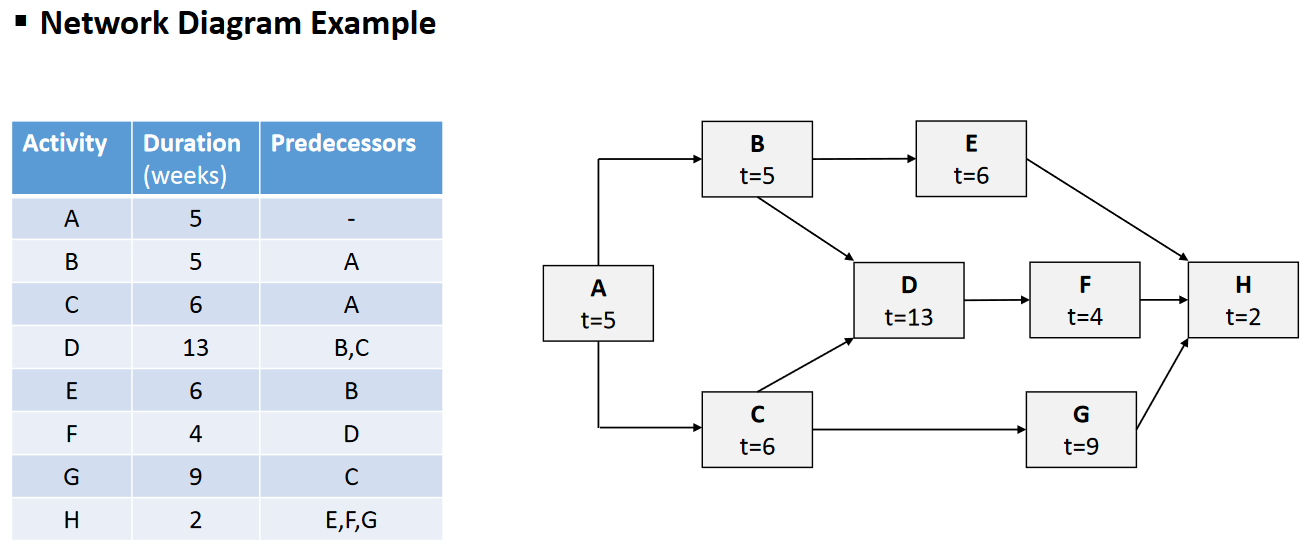
\includegraphics[width=\linewidth]{network_diagram_example.png}
\end{figure}

Early Start (ES) date: the earliest possible date on which an activity can start (based on predecessors)

Late Start (LS) date: the latest possible date that an activity may begin without delaying the project (or a
milestone)

Merge Activity: an activity with two or more immediate predecessors (tasks flowing in)

Burst Activity: an activity with two or more immediate successors (tasks flowing out)

Float (aka Slack, Total Float): The amount of time an activity may be delayed from its early start without
delaying the finish of the project. Float = (LS-ES) or (LF-EF)

\begin{figure}[h!]
  \centering
  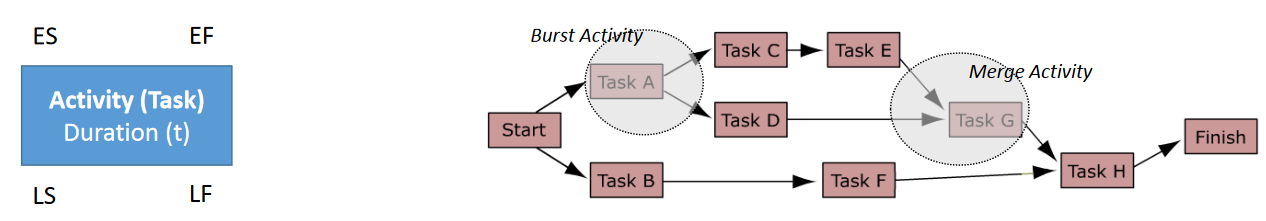
\includegraphics[width=\linewidth]{network_diagram_definitions.png}
\end{figure}

\newpage

\begin{figure}[h!]
  \centering
  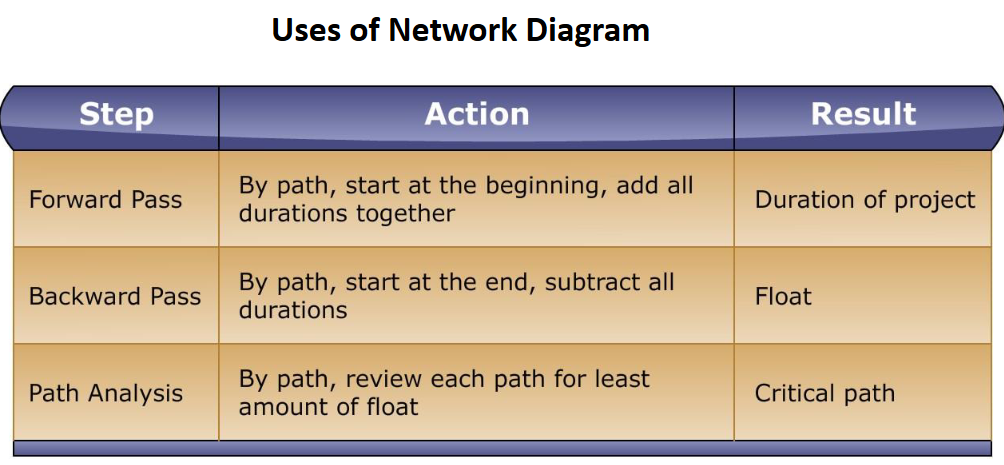
\includegraphics[width=\linewidth]{uses_of_network_diagram.png}
  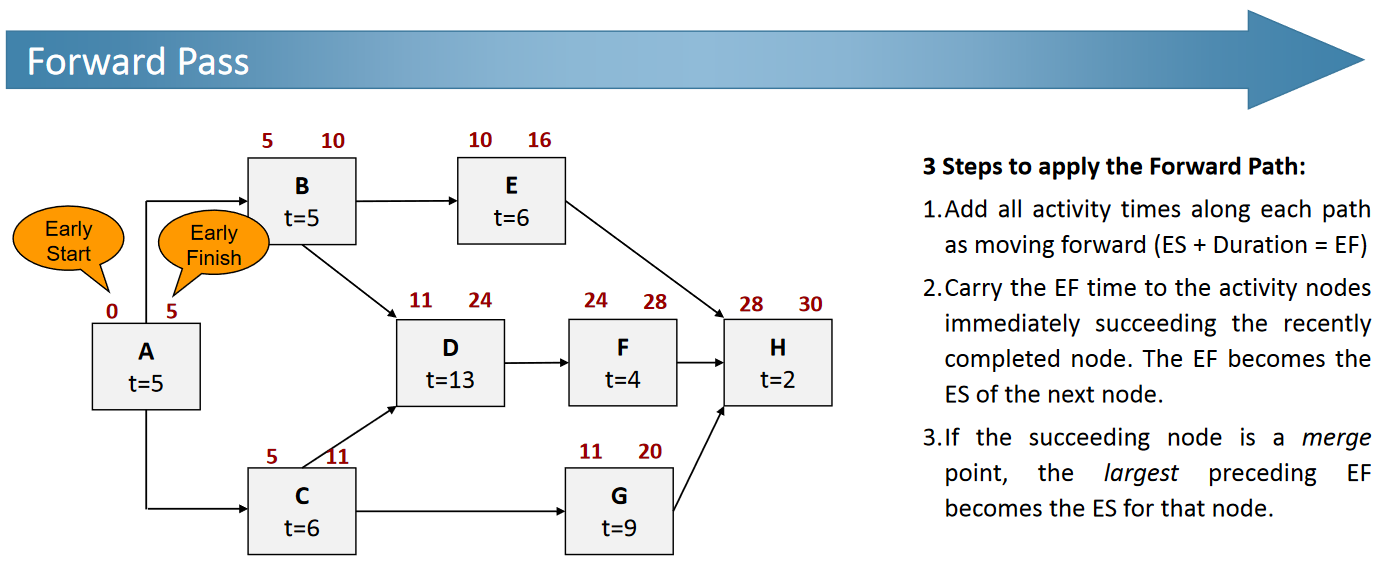
\includegraphics[width=\linewidth]{network_diagram_forward_pass.png}
  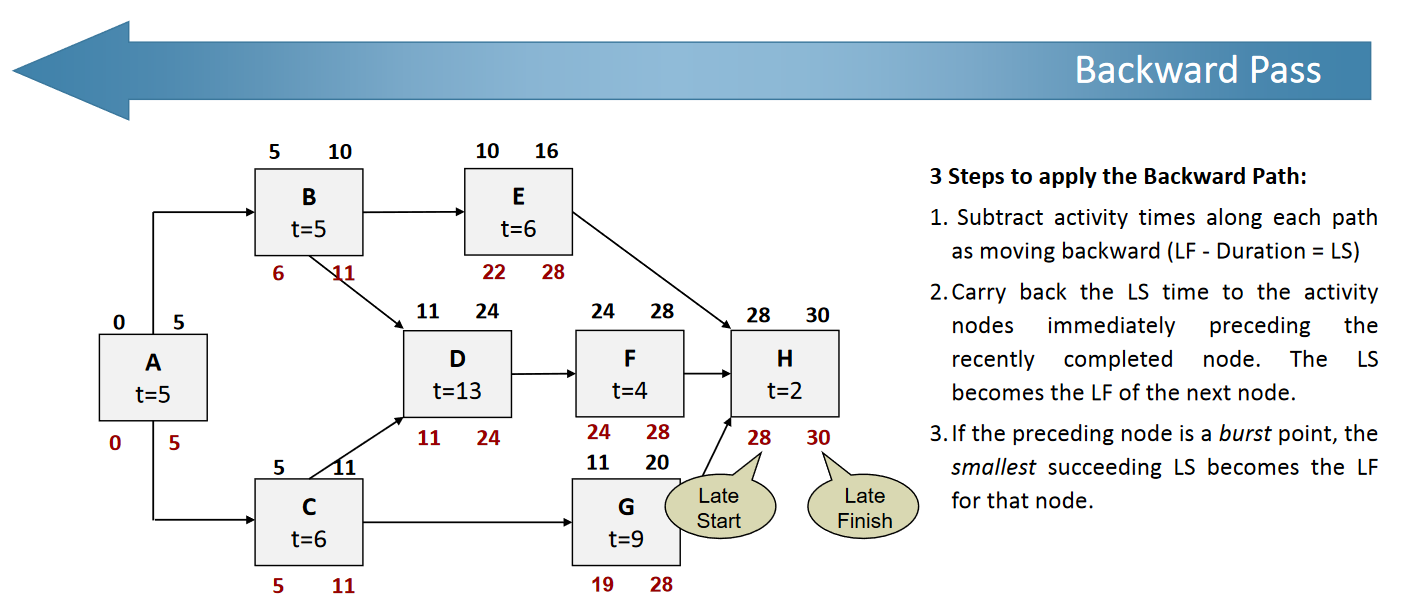
\includegraphics[width=\linewidth]{network_diagram_backward_pass.png}
\end{figure}

\newpage

\begin{figure}[h!]
  \centering
  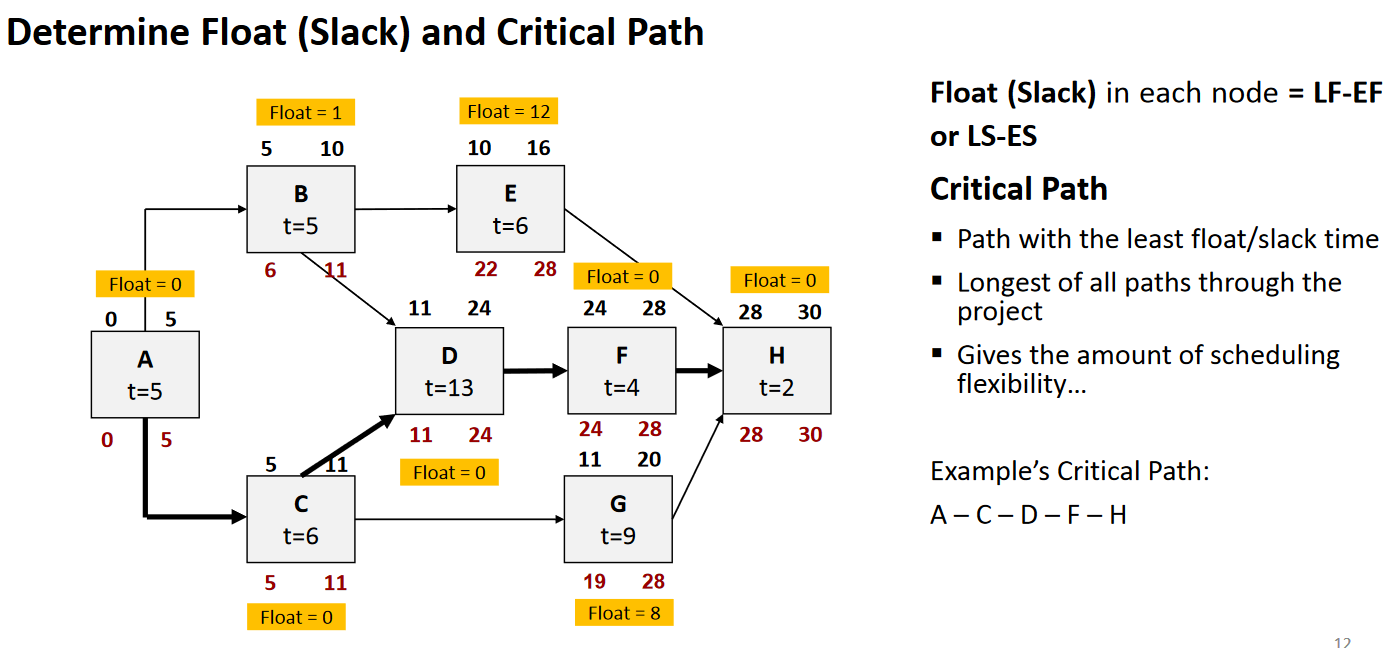
\includegraphics[width=\linewidth]{network_diagram_float.png}
\end{figure}

If LF-EF != LS-ES, your calculation is wrong

Float = 0, means that you cannot delay the task without delaying the entire project\\
(float is in weeks, i.e., if your float = 1 for a task, you can delay that task for 1 week without delaying the project)

Note: we have not included “lags” in our examples and diagrams, e.g. commonly “Finish to Start”,
“Finish to Finish” and “Start to Start”.

Common Options to Shorten the Project/Reduce the Critical Path\\
1. Eliminate Tasks on the Critical Path\\
2. Replan Serial Paths to become Parallel\\
3. Shorten the duration of Critical Path Tasks or of Early tasks\\
4. Shorten Longest tasks\\
5. Shorten Easiest Tasks\\
6. Shorten tasks that cost the least to speed up

\subsubsection{Gantt Charts}
\begin{figure}[h!]
  \centering
  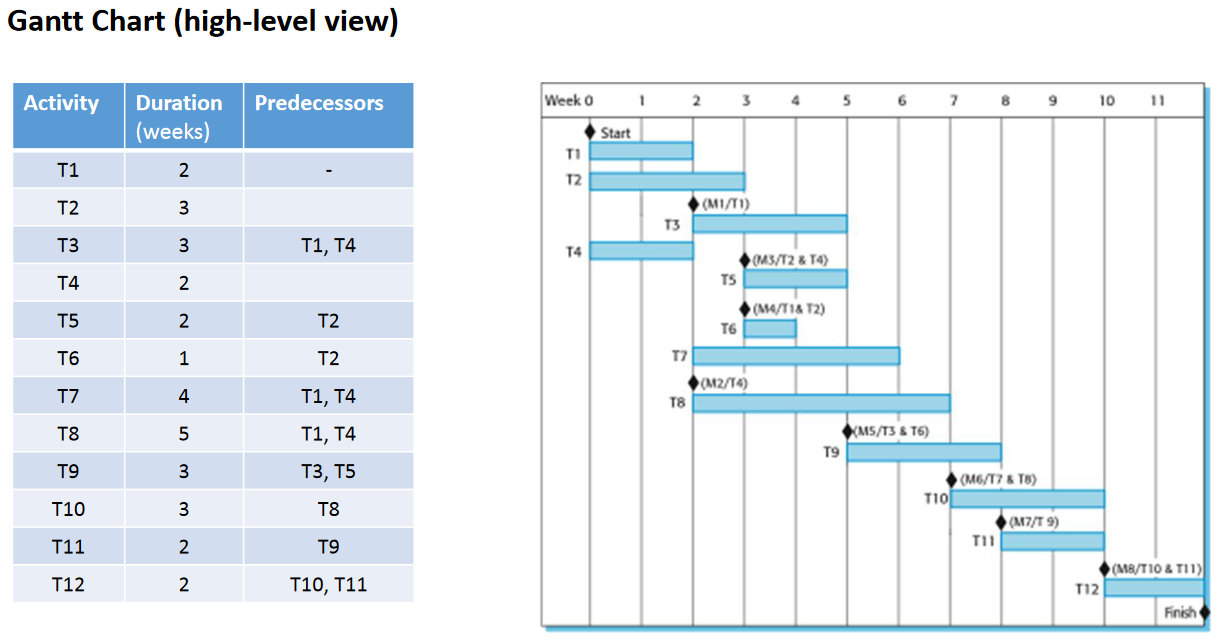
\includegraphics[width=\linewidth]{gantt_chart_example.png}
\end{figure}

\newpage

\subsubsection{Milestones}
Typically part of a Gantt chart (black diamonds on the previous example) and are visual (you have completed something)

\bulletPoint Activities of “zero duration”\\
\bulletPoint Take no time and consume no resources\\
\bulletPoint Record significant events or deliverables\\
\bulletPoint Major project happenings (component X complete)\\
\bulletPoint Funding points (30\% of budget expended)\\
\bulletPoint Key Dates (e.g. system rollout)\\
\bulletPoint Serve as reminders to check on overall project status at key points

Common Options typically applied to accelerate (crash) a Project\\
(all of which have difficulties/drawbacks/ consequences)\\
1. Improve Productivity of Existing Project Resources\\
2. Change Working methods employed - \\initially slows you down (e.g., time to setup a new tool)\\
3. Reduce Scope (how about reducing Quality?)\\
4. “Fast Track” the Project (see relevant discussion in Critical Path)\\
5. Overtime Work (is this a good idea? - cannot be the rule, only the exception - there will be burnout)\\
6. Add Resources to the Project Team (but do not forget the “Brook’s Law” - if you add people to an already delayed project, you are very likely to delay it even further, e.g., onboarding takes time out of new and old developers)

\section{Resources}

Plan for the resources that are required to successfully carry out the project

Main Types of Resources:\\
\bulletPoint People, with specific Skills -> who will do what?\\
\bulletPoint Equipment (incl. all elements of the HW infrastructure),\\
\bulletPoint Software Infrastructure and Tools,\\
\bulletPoint Facilities (e.g. Space)

Primary Inputs:\\
\bulletPoint The activity list and corresponding resource requirements\\(e.g. skills, infrastructure, tools, equipment)\\
\bulletPoint The Project Stakeholders Analysis and Governance Structure and Roles\\
\bulletPoint Resources’ Availability\\
\bulletPoint Trade-off between tasks Time and Resources (an iterative process)\\
\bulletPoint Personalities, Experience, Group Dynamics, People Growth\\
\bulletPoint Related Risks

Key Question: How will I get the best resources and use who I have as best as I can?

\newpage

Example Resource Requirements Analysis
\begin{figure}[h!]
  \centering
  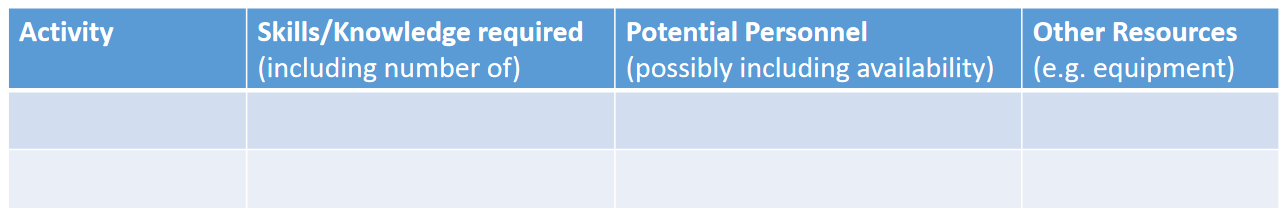
\includegraphics[width=\linewidth]{resource_requirements_analysis.png}
\end{figure}

\subsection{Responsibility Matrix}
or RACI matrix
\begin{figure}[h!]
  \centering
  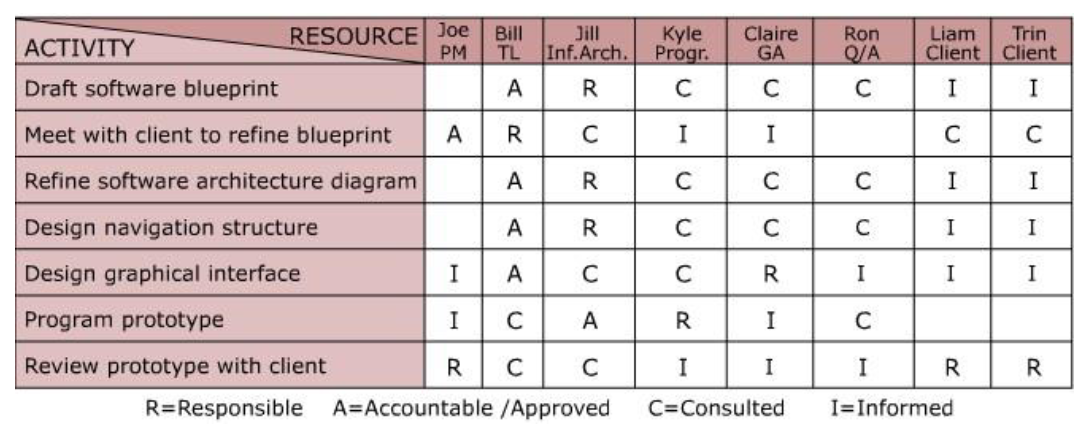
\includegraphics[width=\linewidth]{raci_matrix.png}
\end{figure}

Responsibility is someone doing the activity\\
You can have an A and a R together in the matrix

You can transfer responsibility but not accountability

\subsection{Resource Gantt Chart}

\begin{figure}[h!]
  \centering
  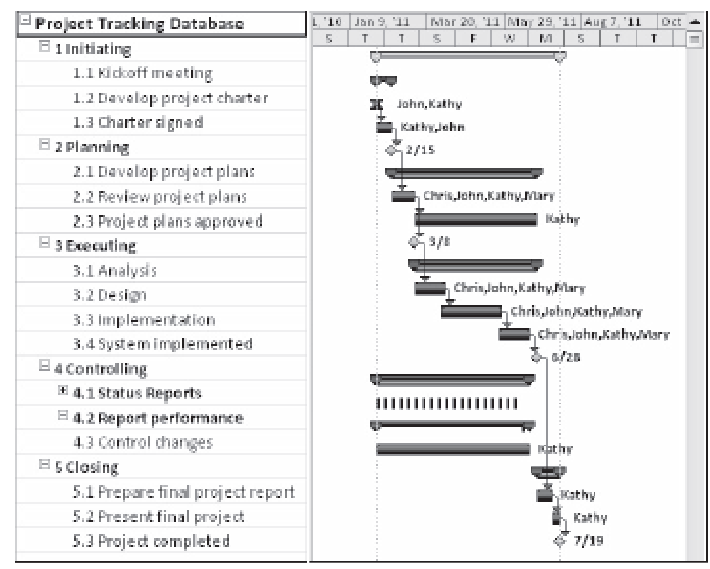
\includegraphics[width=20em]{resource_gantt_chart.png}
\end{figure}

A gantt chart that also shows the resources working on the task

\newpage

\subsection{Resource Loading Histogram}
The amount of individual resources that an existing
schedule requires over time

\begin{figure}[h!]
  \centering
  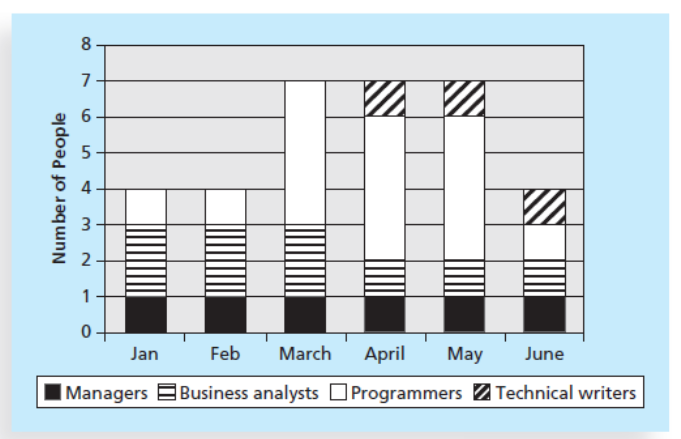
\includegraphics[width=30em]{resource_loading_histogram.png}
\end{figure}

\subsection{Resource Loading Table}
Item in red indicates resource overallocation

Resource Leveling: resolving resource conflicts (incl. overallocation) or achieving a smoother distribution of
resources (mainly by delaying tasks based on their slack)

\begin{figure}[h!]
  \centering
  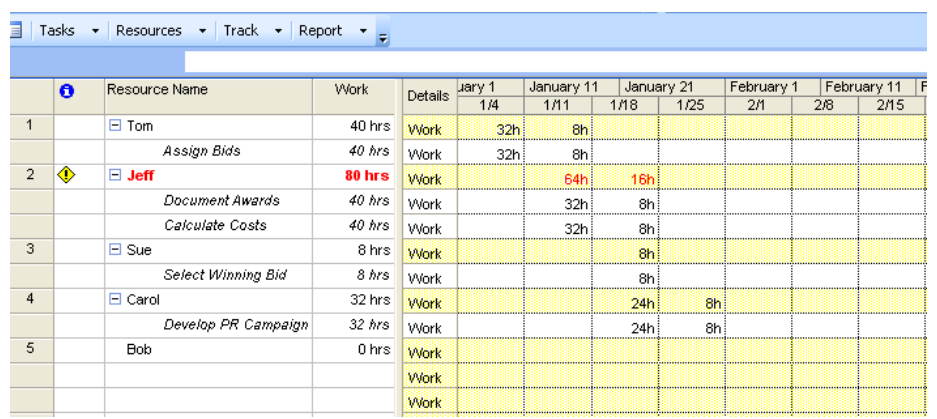
\includegraphics[width=\linewidth]{resource_loading_table.png}
\end{figure}

\newpage

\section{Communications}

Communications Management:\\
The processes required to ensure timely and appropriate generation,
collection, distribution, storage, retrieval and disposition of project information.

Goal is that essential knowledge is passed to team members and stakeholders so that decisions are based on accurate and
complete information.

Communications Plan: a document that describes project communications. Addresses the following items:\\
\bulletPoint Stakeholders Communications Requirements\\
\bulletPoint Information to be communicated, incl. format, content and level of detail\\
\bulletPoint Who will receive the information and who will produce it\\
\bulletPoint Methods (e.g. reports, meetings) or technologies to distribute the information\\
\bulletPoint Frequency of Communication\\
\bulletPoint Escalation Procedures for Resolving Issues\\
\bulletPoint Revision procedures for updating the communications management plan\\
\bulletPoint Project Archives Information\\
\bulletPoint Lessons Learned (shared across the organization)\\
\bulletPoint Glossary/Terminology

Answers the questions: What (information), Where (it will come from), Who, When?

Communications Plan Sample Template:
\begin{figure}[h!]
  \centering
  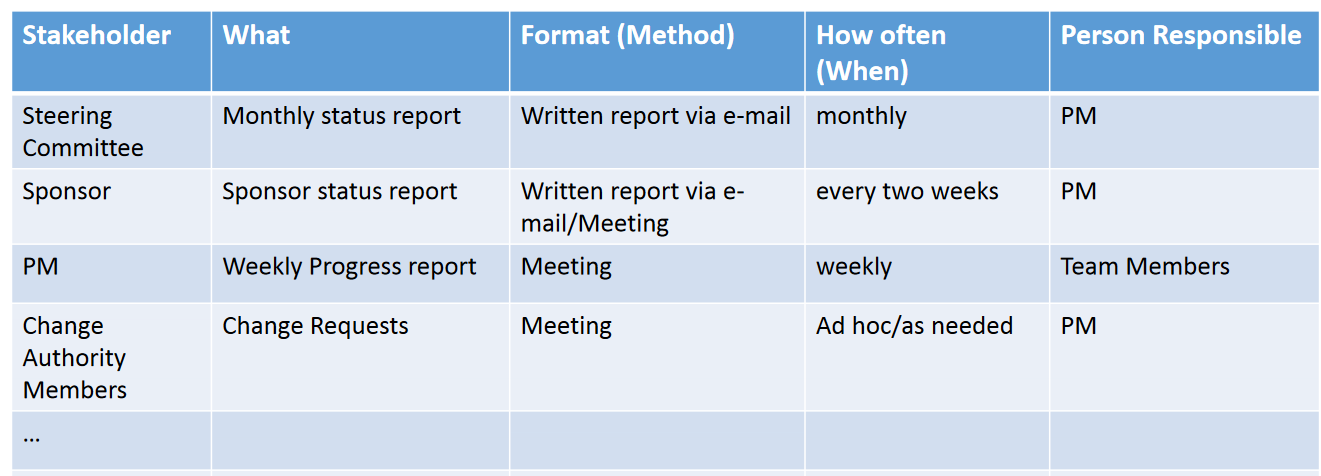
\includegraphics[width=\linewidth]{communications_plan_sample.png}
\end{figure}

\newpage

Typical project meetings:

\textbf{Kick-off Meeting} (discussed – at end of initial planning or at end of full planning)

\textbf{Core Team Project Meetings}:\\
\bulletPoint PM is responsible for determining frequency (e.g. weekly or ad-hoc) and preparing/organizing\\
\bulletPoint Every member of the project’s core team should participate (or representatives in larger projects)\\
\bulletPoint Agenda: accomplishments since the last meeting, status vs work plan, outstanding items since the last meeting, issues and
resolution planning, scope/changes, risks, conclusions and actions items.\\
\bulletPoint Meeting minutes are documented and distributed to the whole team. Changes may have to be made to schedule/plans etc.

\textbf{Project Status and/or Progress Reports and/or Meetings}\\
(typically regularly scheduled)\\
\bulletPoint Status: where the project stands at a particular point in time (e.g. schedule, costs, scope)\\
\bulletPoint Progress: what has been accomplished during a certain period (e.g. a month), plans for the next period, issues, risks,
projected/proposed actions, changes, forecasting (predicting future status/performance)

Different reports/meetings of such type may take place: with Sponsor, with key-stakeholders (e.g. Business Units), Steering Committee.
Meeting minutes are documented and distributed. Changes may have to be made to schedule/plans etc.

\textbf{Ad Hoc Meetings}\\
Plan who will organize, attend, etc. What will be distributed before and after, etc.

\textbf{Project Closure Meeting}: to formally closeout the project. Agenda: Post-implementation audit, lessons-learned,
release of resources, formal acceptance, celebration.

\begin{figure}[h!]
  \centering
  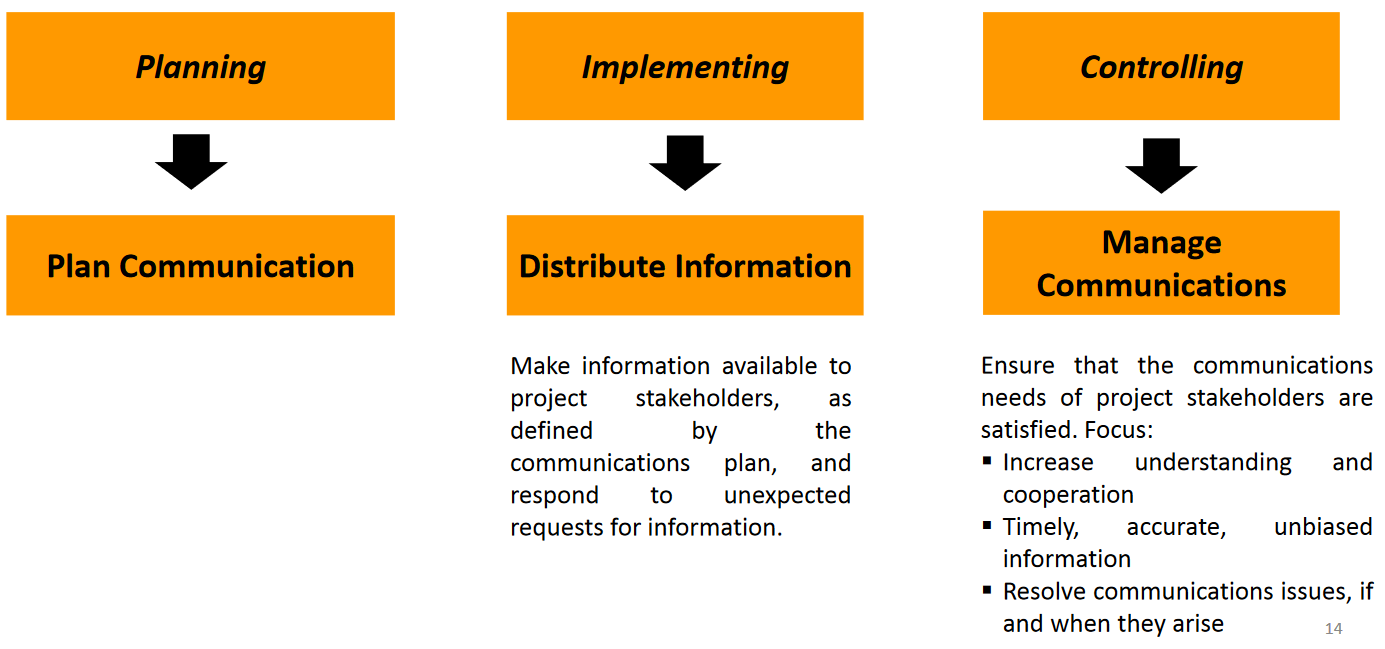
\includegraphics[width=\linewidth]{communications_stages.png}
\end{figure}

\chapter{Risk management}

What is a Risk?\\“An uncertain event or condition that, if it occurs, has a positive or a
negative effect on a project’s objective” or “uncertainty of outcome” (Prince2)

Characteristics of a Risk:\\
\bulletPoint A definable event\\
\bulletPoint Probability of occurrence\\
\bulletPoint Impact (consequence) of occurrence

A degree of risk-taking is inevitable in projects.

An issue is something that is already reality

What is Risk Management?\\ “Manage a project’s exposure to risk (that is, the probability of
specific risks occurring and the potential impact if they did occur). The aim is to manage that
exposure by taking action to keep exposure to an acceptable level in a cost-effective way.”

What is Risk Tolerance or Risk Appetite?\\ The amount of risk a project is prepared to
tolerate (typically considered by PM, Project Sponsor and SC, taking into account the
overall organization’s risk tolerance).

What is a Risk Management Plan?\\ Documents the procedures for managing risks
throughout the project, i.e. how risk management will be performed on the project. Part
of the overall Project Management Plan.

Main topics addressed in a Risk Management Plan:\\
1. (Monitoring) Methodology\\
2. Roles and Responsibilities (Who is responsible for what)\\
3. Budget and Schedule (e.g., contingency reserves)\\
4. Risk Categories\\
5. Risk Probability and Impact\\
6. Risk Tolerances\\
7. Risk Tracking and Documentation

Generic Risk Management process:
\begin{figure}[h!]
  \centering
  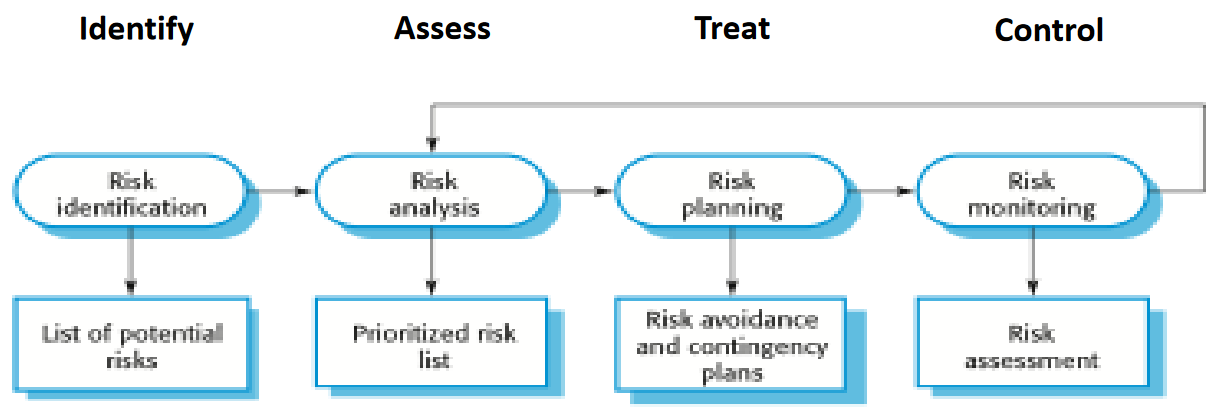
\includegraphics[width=\linewidth]{generic_risk_management_process.png}
\end{figure}

\newpage

Risk analysis; evaluate probability and impact

Risk planning; in a cost effective way

\section{Risk Identification}

Identify Threats (negative impact) or opportunities (positive impact). A repeatable process as
a risk may change or new risks may emerge during the project.

Can be done via brainstorming, interviewing, workshops or individually (e.g. PM), checklists,
previous projects, Risk Breakdown Structures.

Project post-mortem; looking at failed projects and what went wrong\\
Project pre-mortem; bringing in the project team and imagining what could have gone wrong from an impact (working backwards)

Involved multiple participants, e.g. PM, Project Sponsor, SC, Project Team, senior managers,
users, risk management experts, subject matter experts.

Risks should be specific, e.g. of the form: If <event> when <point in project> then <result>

The primary output are relevant entries in a Risk Register (or else known as Risk Log
(Prince2))

\begin{figure}[h!]
  \centering
  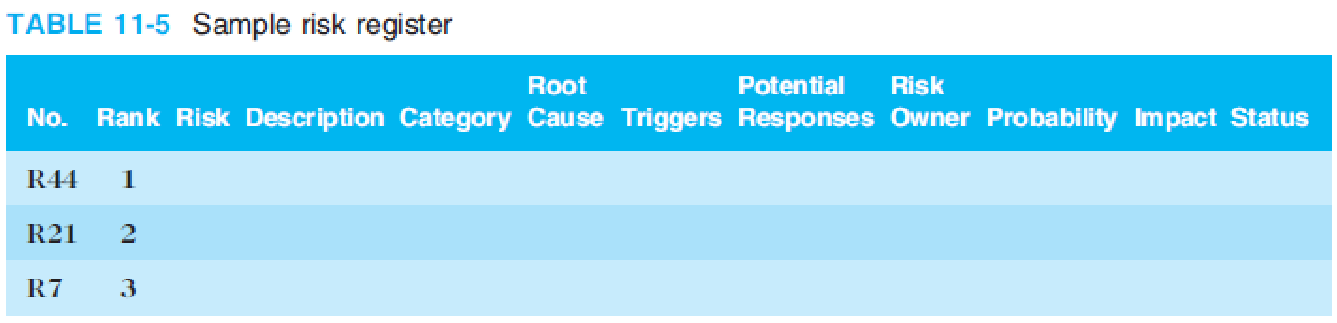
\includegraphics[width=\linewidth]{risk_register.png}
  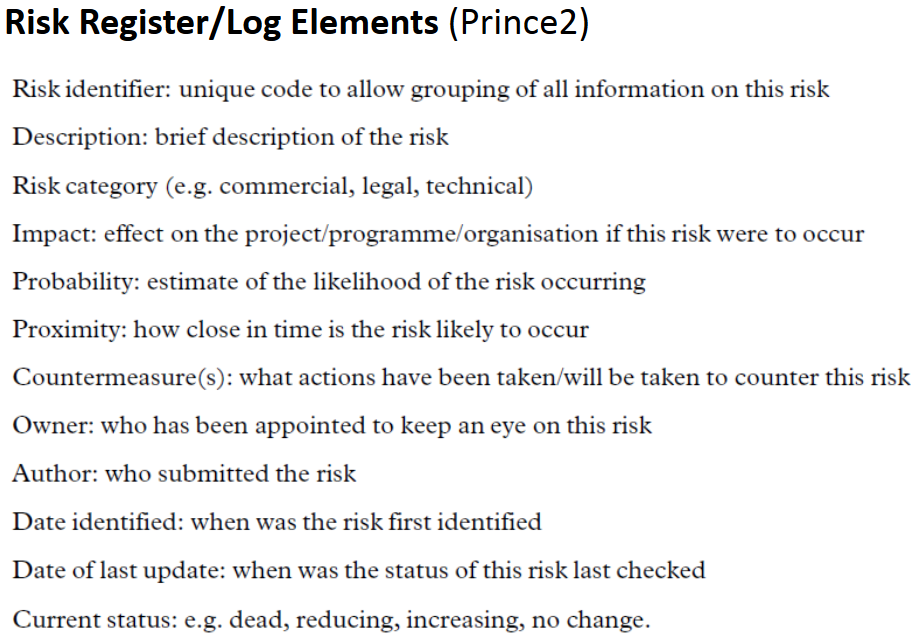
\includegraphics[width=30em]{risk_register_prince2.png}
\end{figure}

\newpage

\section{Assess (Risk Analysis)}
Measure and prioritize the risks for further action.

This process includes estimating the probability of
occurrence of each risk and the corresponding
impact for project objectives, if the risk does occur.

The risks are then prioritized in accordance with
this assessment considering other factors such as
the timeframe and key stakeholders’ risk tolerance.

Impact is often considered in terms of time,
quality, cost/benefit, people/resources.

Impact scale can be H/M/L or catastrophic, serious,
tolerable or insignificant (or other similar scales)

Risks may be quantified (using a number of
methods)

\begin{figure}[h!]
  \centering
  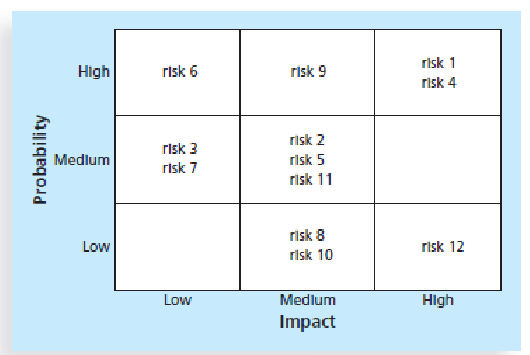
\includegraphics[width=30em]{risk_analysis_matrix.png}
\end{figure}

\newpage

\section{Treat (Planning)}
Develop options and determine actions to reduce threats to project
objectives.

Actions typically break into the following 5 types (from Prince2)

\begin{figure}[h!]
  \centering
  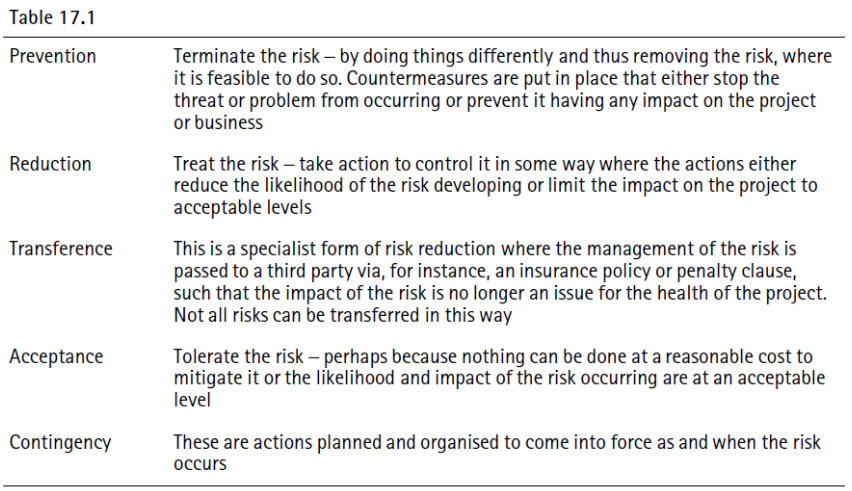
\includegraphics[width=40em]{risk_actions.png}
\end{figure}

\textbf{Note.} Treating risks implies including resources and activities into the
project’s budget and schedule. Risk treatment should be appropriate to the
risk, cost-effective, timely, realistic within the project context, understood
by all parties involved and assigned to an appropriate person.

\section{Control (Monitoring)}
Purpose is to minimize disruption to the project by determining whether the risk
responses are executed and whether they have the desired effect.

It is achieved by tracking the identified risks, identifying and analysing new risks,
monitoring trigger conditions for contingency plans and reviewing progress on risk
treatments while evaluating their effectiveness.

Project risks should be periodically evaluated throughout the project life cycle, when a
new risk arises or when a milestone is reached.

\newpage

\section{Main Responsibilities}

\textbf{Project Manager:}\\
Responsible for the overall management of risk (a key-responsibility), including identifying risks herself.

The PM should “eat, sleep and breath” with potential risks and risk management. Apart from considering uncertain events or conditions, key
questions also include: “What we have not been doing, and we should have been doing (or plan to do)?” and “What are
possible consequences of what we have been or not been doing?”

\bulletPoint Ensures that risks are identified, recorded and regularly reviewed.\\
\bulletPoint Modify project plan to include risk management.\\
\bulletPoint Timely communication is a critical success factor!

\textbf{Project Teams:}\\
Proactively identify risks and timely alert the Project Manager. Actively participate in treatment actions.

\textbf{Project Steering Committee and/or Project Sponsor:}\\
\bulletPoint Notify PM of any external risk exposure\\
\bulletPoint Make decisions on recommended by the PM actions to risk\\
\bulletPoint Balance risk-taking and benefits of the project\\
\bulletPoint Notify programme management and/or organization of any risks that affect project’s ability to meet corporate or
programme objectives.

\begin{figure}[h!]
  \centering
  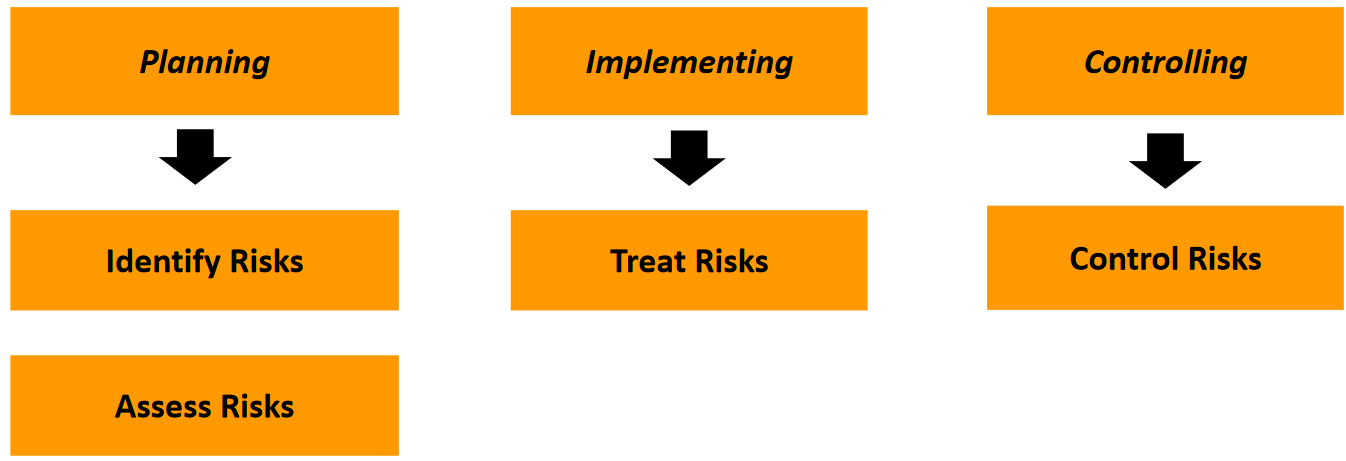
\includegraphics[width=\linewidth]{risk_management_stages.png}
\end{figure}

\chapter{Project Controlling / Monitoring}

\section{Configuration Management}

Configuration management (CM) is concerned with the policies, processes and
tools for controlling and managing assets or products.

Assets/Products include a number of artifacts, both Project and Systems’
related, e.g. source code, executables, component libraries, files,
documentation, manuals, project-related documents.

Typical concerns: Change Control and Versions, Status, Ownership,
Relationships, Safe and Secure Storage.

Note that Project-Level CM is different to Organization-Level CM, however the
former should be consistent with the policies and practices of the latter.

\textbf{Configuration Item (CI):}\\Any artifact (e.g. design, code, test scenarios, document, etc.) that has been
placed under configuration control, i.e. ensuring that versions are recorded and maintained and all
versions are identified and stored for the lifetime. There are often different versions of a configuration
item. Configuration items have a unique name.

Deciding what level of configuration management will be required in a project (or in the overall
organization) and planning how this level is to be achieved is an important planning consideration.

\textbf{Version:}\\An instance of a configuration item that differs, in some way, from other instances of that item.
Versions always have a unique identifier, which is often composed of the configuration item name plus a
version number.

\textbf{Version management:}\\Keeping track of the multiple versions of assets/products and ensuring that changes
made (e.g. by different developers) do not interfere with each other.

A \textbf{Codeline} is a set of versions of a software component and other configuration items on which that
component depends.

A \textbf{Baseline} is a snapshot of the state of a product and any component products, frozen at a point in time for
a particular purpose. For example, when the Project Plan is agreed between Project Manager and Project
Board, it is ‘baselined’.

In SW terms, a baseline is a frozen collection of component versions that make up a system. Baselines are
controlled, which means that the versions of the components making up the system cannot be changed.
This means that it should always be possible to recreate a baseline from its constituent components.

\newpage

\textbf{Change management:}\\Keeping track of requests for changes to the assets/products (e.g. software from
customers and developers), working out the costs and impact of changes, deciding the changes should be
implemented and track changes – (see next section)

\textbf{System building:} The process of assembling program components, data and libraries, to create an
executable system.

\textbf{Release management:}\\A release is a complete and consistent set of products, which forms a fixed
reference point in the development of the end outcome, e.g. a system version ready to become available to
end-users. Release Management mainly concerns planning, preparing and tracking product versions for
release.

\begin{figure}[h!]
  \centering
  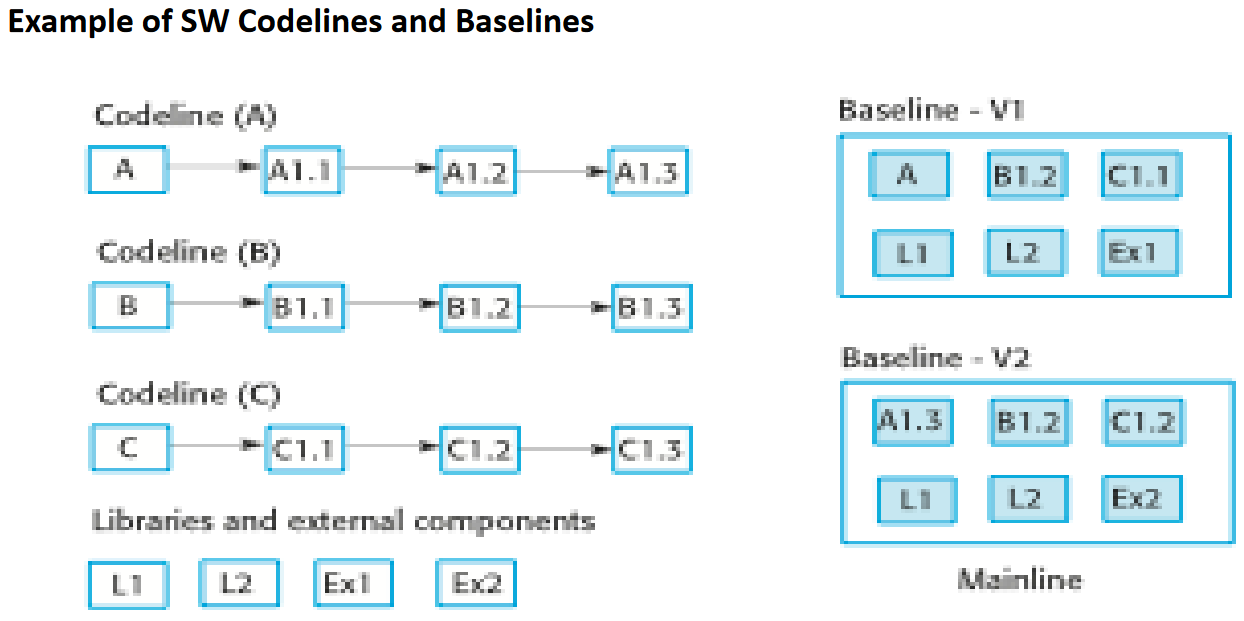
\includegraphics[width=\linewidth]{codelines_and_baselines.png}
  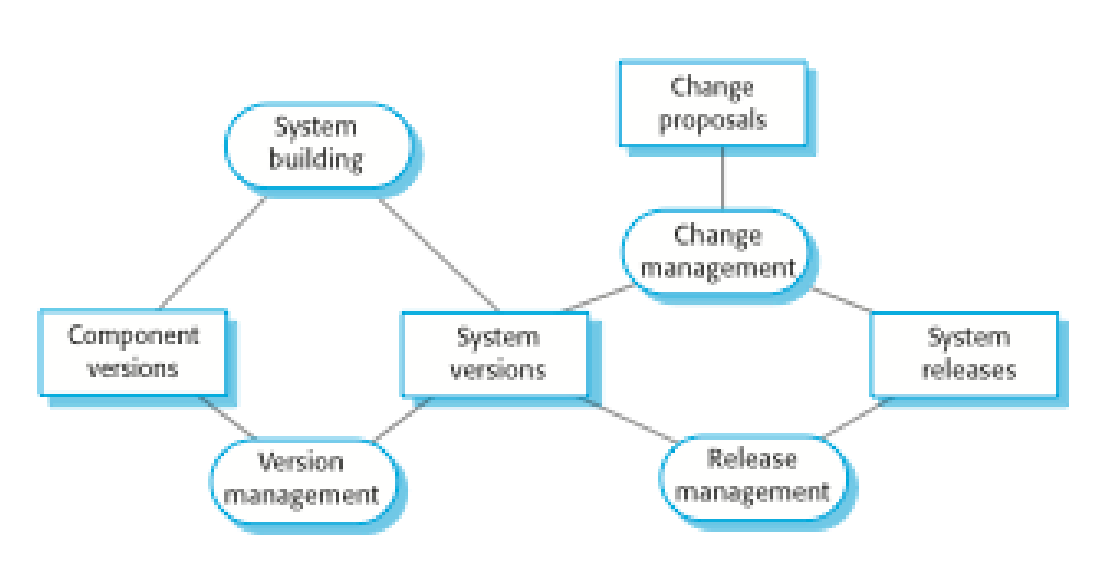
\includegraphics[width=\linewidth]{configuration_management.png}
\end{figure}

\newpage

\subsection{Change management}
A process that manages change, i.e. “the assessment of the impact of potential changes,
their importance, their cost and a judgmental decision by management on whether to include them or not. Any
approved changes must be reflected in any necessary corresponding change to schedule and budget.” (Prince2)

Changes are associated to Project Issues, i.e. anything that could have an effect on the project. For example:\\
\bulletPoint Change in Requirements\\
\bulletPoint A change in the Project Environment such as: a legislative change, a new stakeholder, an unexpected change
to a member of the project team, a programme management directive, a corporate reorganisation\\
\bulletPoint A problem occurring or being identified that was not anticipated during risk analysis\\
\bulletPoint Problem or error occurring in work completed or currently under way

Project Issues are typically captured in an Issue Log, are assessed to determine/plan actions and reviewed to
monitor progress. Issues are also related to Risks (How?)

Issues/Changes Assessment, Actions and Review are often performed by a Change Control Board (CCB) (e.g.
the Project SC (Project Board) or to a delegate body). In Prince2 this is known as “Change Authority”.

Changes formally originate via formal Change Requests (CR). The set of CRs are maintained in a relevant Log

\begin{figure}[h!]
  \centering
  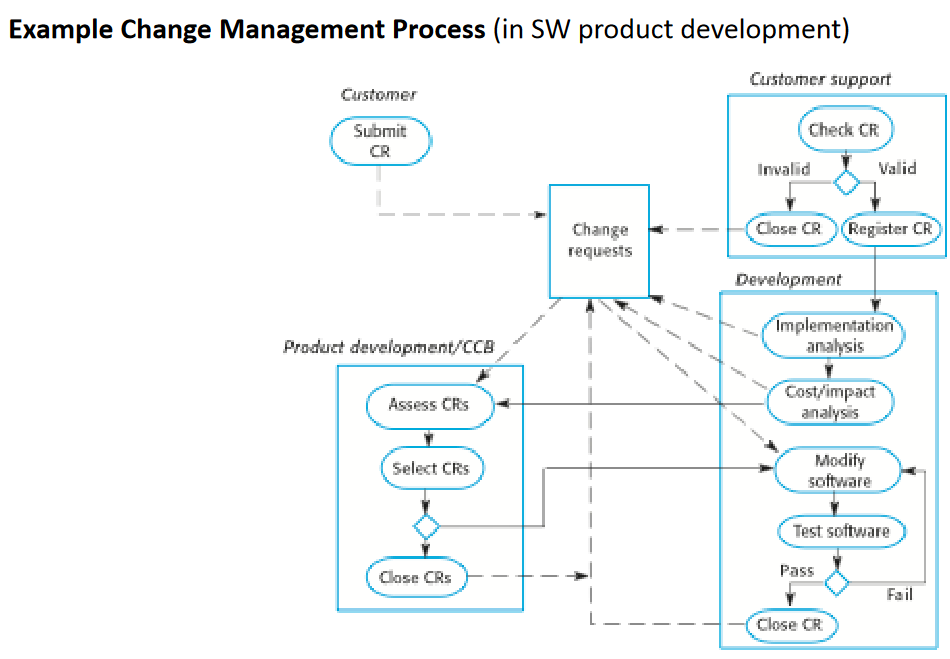
\includegraphics[width=\linewidth]{change_management_process.png}
\end{figure}

\newpage

\begin{figure}[h!]
  \centering
  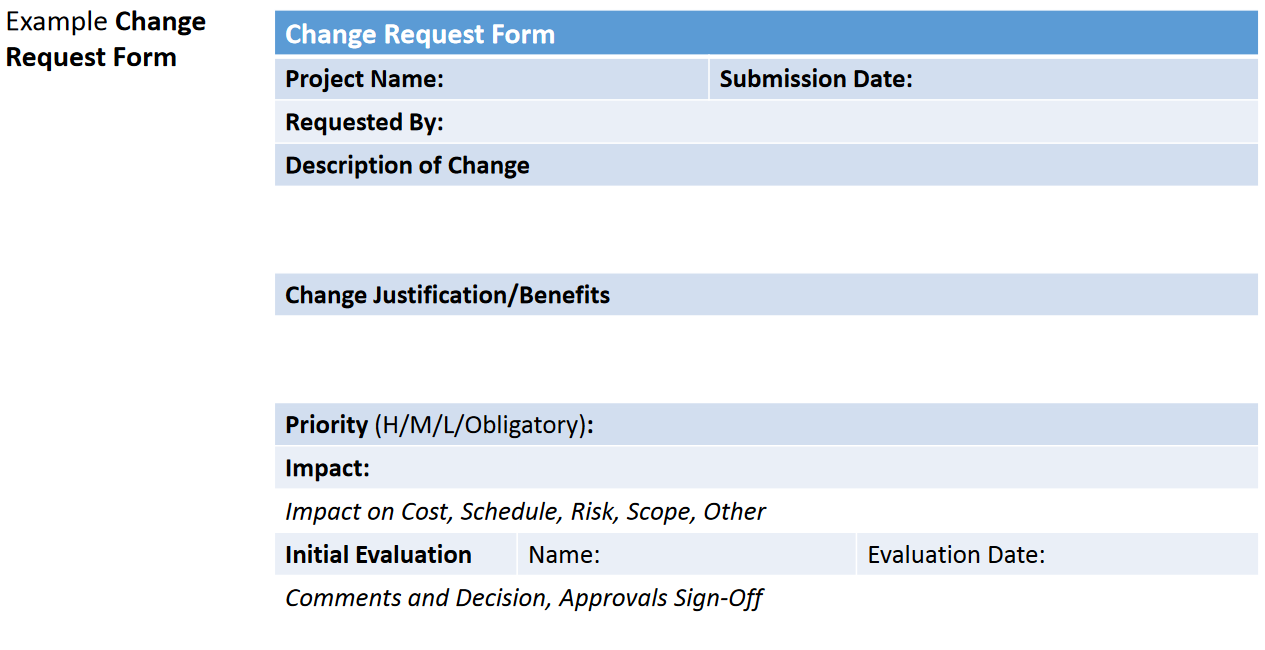
\includegraphics[width=\linewidth]{change_request_form.png}
  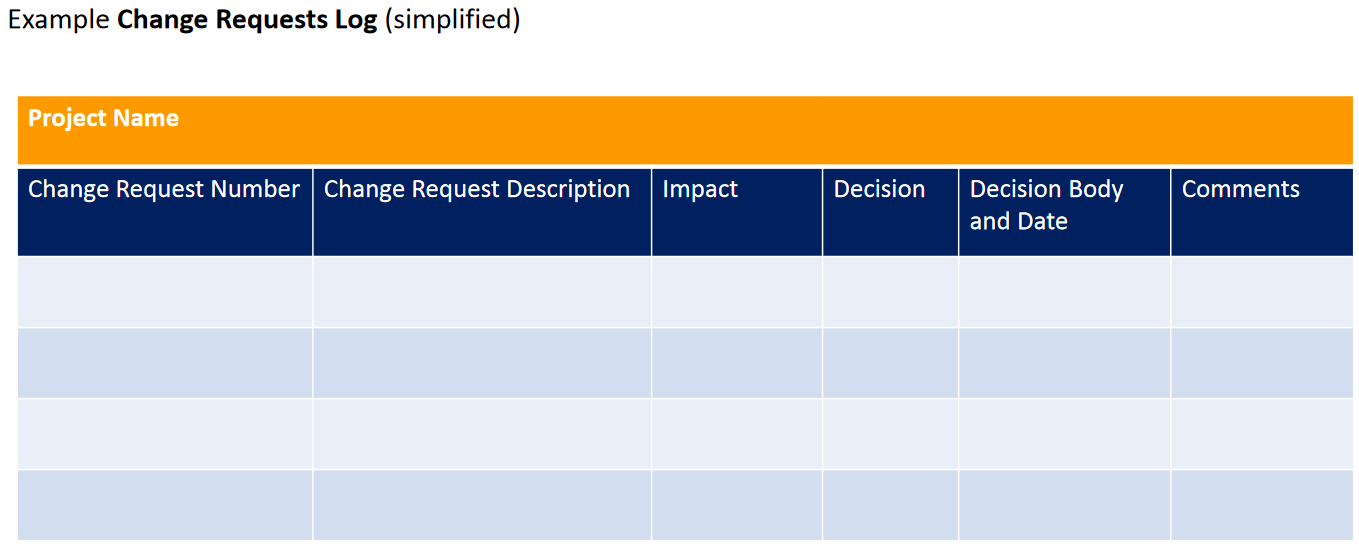
\includegraphics[width=\linewidth]{change_requests_log.png}
  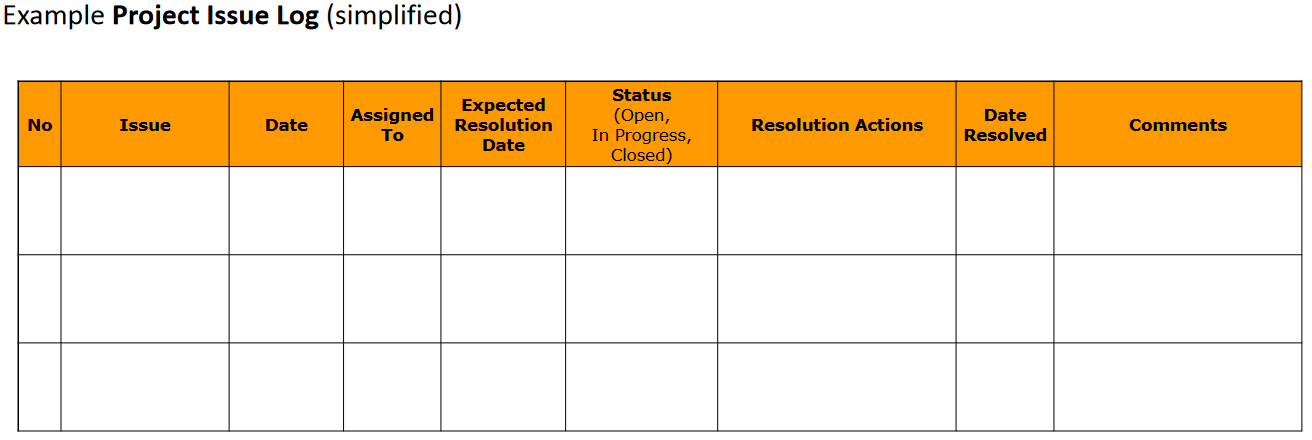
\includegraphics[width=\linewidth]{project_issue_log.png}
\end{figure}

Note: Each organization/project typically has its own concrete change management process, with
associated roles, responsibilities, tasks and document templates

\newpage

\section{Control Project Progress/Performance}

\textbf{Control Schedule} (ISO 21500): The purpose of Control Schedule is to \textbf{monitor schedule variances} and to \textbf{take
  appropriate actions}. This process should \textbf{focus on determining the current status of the project schedule},
\textbf{comparing it to the approved baseline} schedule to determine any variance, \textbf{forecasting completion} dates and
\textbf{implementing any appropriate actions} to avoid adverse schedule impacts. All changes to the baseline schedule
should be managed in accordance with Change Management processes.

\textbf{Control Costs} (ISO 21500): The purpose of Control costs is to \textbf{monitor cost variances} and to \textbf{take appropriate
  actions}. This process should \textbf{focus on determining the present project cost status}, \textbf{comparing it to the baseline}
costs to determine any variance, \textbf{forecasting projected costs at completion} and \textbf{implementing any appropriate
  preventive or corrective actions}, in order to avoid adverse cost impacts. All changes to the baseline costs
should be managed in accordance with Change Management processes.

Once work is started, performance data are accumulated including budgeted costs, actual costs and estimated
cost at completion.

In order to evaluate cost performance it is necessary to accumulate scheduling data, such
as the progress of scheduled activities and the forecasted completion dates of current and future activities.

\textbf{Variances} might arise from poor planning, unforeseen scope changes, technical problems, equipment failures
or other external factors, such as supplier difficulties. Regardless of the cause, corrective actions require either
a change in the cost baseline or the development of a short-term recovery plan.

The main methods / tools to control project performance;\\
1. S-Curve Analysis (focus on Cost vis-a-vi Schedule)\\
2. Milestones (focus on Schedule)\\
3. Tracking Gantt Charts (focus on Schedule)\\
4. Earned Value Management (a more holistic approach)\\
5. Scrum/Agile: Velocity and Sprint/Release Burndown Charts

\subsection{S-Curve Analysis}

Focus on Cost vis-{\`a}-vis Schedule

Advantages: Simple, Clear, easy to update\\
Main Issue: may be misinterpreted and not “tell” the whole truth on project actual performance

\begin{figure}[H]
  \centering
  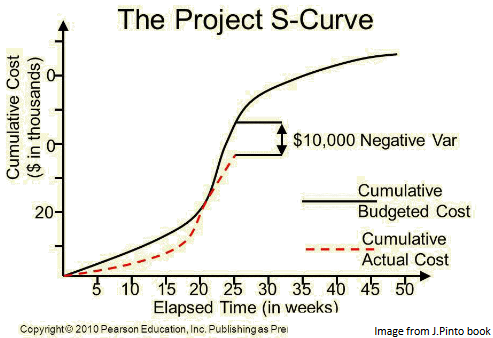
\includegraphics[width=.6\linewidth]{s curve analysis.png}
\end{figure}

The 10k negative variance, means that we are spending less than budgeted /
expected for. This may or may not be a good thing; it could mean we are being
more cost-efficient than expected, or it could mean that we are spending less
due to not making good progress.

This example shows that the tool is more of a starting-point to tell us to
dig further and figure out what is going on

\subsection{Milestones}

Focus on Schedule

Advantages: Simple, Clear, Widely Used.\\
Main Issue: they are Reactive,\\
i.e., if a milestone has a certain date to
complete a task, and you check on this tool 3 days before and realize that you
will not complete the task, then it is already too late and you cannot easily recover

A milestone is a specific point in time. We call it a task but it is an
activity with no duration of effort and signals important points in time in a
project, e.g., end of testing.

We can control performance by looking at milestones and checking whether we have
achieved them. Used especially when reporting things back to upper management.

\subsection{Tracking Gantt Charts}

Focus on Schedule

Advantages: Easy to understand and updated\\
Issues: Do not show underlying issues, do not easily allow for projections in the future

When you add percentages of completion to a Gantt chart, it becomes a tracking
gantt chart.

Another issue of these is figuring out how to provide a percentage; you sometimes
cannot tell, due to a delay, whether, for e.g., the last 10\% of a task will
take longer than the first. Do you give the percentage as work done for the task
or time taken, out of the total expected?

\begin{figure}[H]
  \centering
  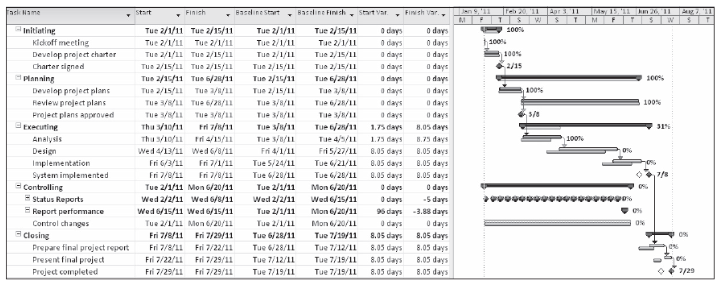
\includegraphics[width=\linewidth]{tracking gantt chart.png}
\end{figure}

\subsection{Earned Value Management (EVM)}

A more established (proper), complex methodology\\
because it is more complex, it is less likely to be used as it is more
rigorous, disciplined and consistent, especially due to the speed some
projects need to go at.

4 variables to consider;\\
\bulletPoint \textbf{PV (Planned Value)}: the budget (or the baselined cost) (up to the current point in time)\\
\bulletPoint \textbf{AC (Actual Cost)} (cumulative)\\
\bulletPoint \textbf{EV (Earned Value)}: (estimate) of the value of the work actually completed\\
\bulletPoint \textbf{RP (Rate of Performance)}: ratio of percentage of actual work completed to the percentage of work planned to have completed at any given point in time.

EV = PV (to date) * RP\\
Cost Variance = EV – AC\\
Schedule Variance (SV) = EV – PV\\
Cost Performance Index (CPI) = EV/AC\\
Schedule Performance Index (SPI) = EV/PV

A negative Schedule Variance value implies it took longer than expected to complete the task

If CPI \textless 100\% then over-budget, if CPI \textgreater 100\% then under-budget

If SPI \textless 100\% then behind schedule, if SPI \textgreater 100 then ahead of schedule

\underline{Example:}\\
Suppose a task is planed to take one week and a cost of £10000 (PV). Suppose that it actually took 2 weeks and a
total cost of £20000, of which £15000 in the first week and £5000 in the second week (AC per week). Suppose that the task
was half-way completed by the end of week 1. This implies that RP=50\%.\\
Calculations:\\
\bulletPoint EV = 10000*50\%=5000\\
\bulletPoint Cost Variance = 5000 – 15000 = –10000\\
\bulletPoint Schedule Variance (SV) = 5000 – 10000 = – 5000\\
\bulletPoint Cost Performance Index (CPI) = 5000/15000 = 33\%\\
\bulletPoint Schedule Performance Index (SPI) = 5000/10000 = 50\%\\
Can calculate 2 new values;\\
\bulletPoint Estimate at Completion (EAC) = Baselined Cost at Completion (BAC) / CPI provides a new estimated cost for the project\\
\bulletPoint Estimate Time to Complete = Original Time to Complete / SPI provides a new estimated time for completion of the project

One may produce an earned value chart to track project performance, i.e. example for a 1-year project after 5 months;
\begin{figure}[H]
  \centering
  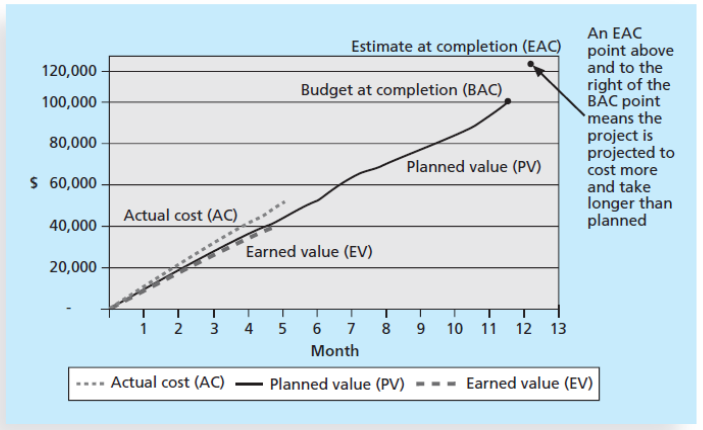
\includegraphics[width=.7\linewidth]{EVM chart.png}
\end{figure}

Concrete Numbers for the EV Graph;
\begin{figure}[H]
  \centering
  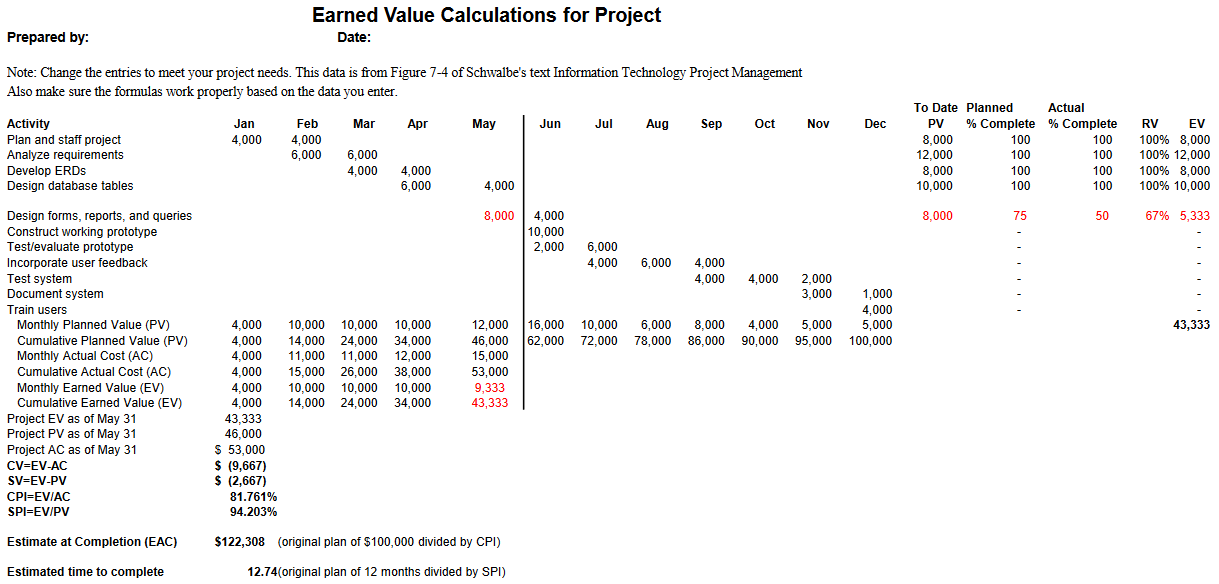
\includegraphics[width=\linewidth]{EVM chart calcs.png}
\end{figure}

The vertical line between May and June shows that we are calculating the end
value at the end of May. We can see the effect of being behind schedule for the
'Design forms, reports and queries' activity on the estimated time to
completion and EAC of the Project.

Many organizations apply a global, uniform rate for budget per day.\\
This has the drawback of not being true to specific roles. Different roles
should have different rates but this is complex so most organizations avoid it
by setting a global rate.

\subsection{Agile}

In scrum/agile, we have some control performance mechanisms

\subsubsection{Velocity}
Cumulative running average of the Story Points delivered in a number of Sprints

Story points are from activities like planning poker

\begin{figure}[H]
  \centering
  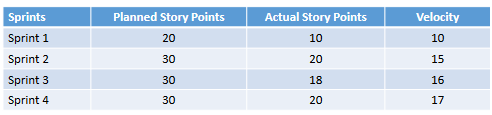
\includegraphics[width=\linewidth]{velocity.png}
\end{figure}

\subsubsection{Burndown Charts}

\begin{figure}[H]
  \centering
  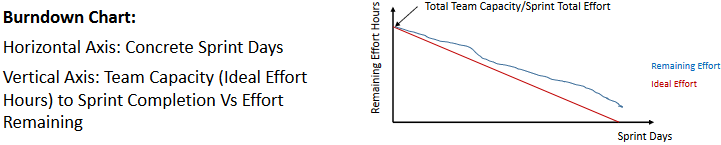
\includegraphics[width=\linewidth]{burdown chart.png}
\end{figure}

Here we can see that the team will probably have to continue the current user
stories in the next sprint. If this continues, the team will be behind schedule.
At that point we consult the project triangle to increase costs or add people, etc.

\section{High-Level Summary of Best Practices}
1. Decide and communicate how you are going to control change, track status and manage issues.\\
(is it going to be a very formal change management process? why? what can everyone (like stakeholders) expect when there are changes? etc.)\\
2. Decide what you will measure.\\
3. Decide how you will measure.\\
4. Risk Control/Management is a key success factor. Evaluate and be proactive!\\
5. Options available are often based on the project triangle\\
6. Quantify options/decisions whenever possible. (be careful of blame games in industry!)\\
7. Recommend and Engage stakeholders Vs Decide\\
(If you make decisions that are not wanted, stakeholders may ask you to repeat work you just did. Over and over until they feel like it is right. It is best you engage them in a timely fashion instead, verifying recommendations by other people in the project, ensuring any challenge to a decision is only a challenge to the process)

\chapter{Fundamentals of Team Management}

 (ISO21500):\\
\textbf{Develop project team} purpose is to improve the performance and interaction
of team members in a continuing manner. This process should enhance team motivation
and performance.\\
The purpose of \textbf{Manage project team} is to optimize team performance,
provide feedback, resolve issues, encourage communication and coordinate changes, in
order to achieve project success.\\
These also depend on the process of actually establishing the Project Team.

But what is a Team? Many definitions, e.g.:\\
“A (small) number of people who are committed to a common purpose and who are
working together and interdependently to achieve specific performance goals using an
approach for which they hold themselves accountable.”

Given that IT Projects are predominantly made by teams of people and their outcomes
are used by people, Team Management (or better Leadership) is probably the most
critical success factor.

People are the hardest factor to get right as they are non-linear

\section{Main Characteristics of effective Project Teams and reasons that teams fail}

\underline{Main Characteristics of effective Project Teams:}

1. A clear sense of Mission\\
People work better if they know how their performance contributes to achieving an objective. Do not use
“mushroom management” (keep them in the dark) or give them isolated/fragmented tasks without
informing on the overall status of the project.\\
It is crucial to invest time to clarify roles and define concrete goals right from the beginning of the project

2. A Productive Interdependency\\
Developing a holistic sense of appreciation for the strengths and contribution of each team
memberto the project success

3. Cohesiveness\\
Degree of mutual “attraction” that team members hold for one another and
their tasks ("being attracted to the fact that they belong to the team"
(due to their tasks))

4. Trust\\
Something very easy to destroy. You should allow openness for counter-arguments;
an atmosphere where people can say what they feel, believe, etc.

5. Enthusiasm\\
Building this is very context-dependant. Try to build and sustain this for as
long as possible.

6. Results Orientation\\
Everyone needs to be focused on the end goal and deliverables. Without this,
the other characteristics do not matter as they will disappear soon

You can’t expect the team to have such characteristics if you, as the PM, do not have them!\\
Leadership is more often leading by example

\underline{Some reasons that Project Teams fail:}

1. Unclear mission \& project/individual goals\\
fragmented, constantly changing, poorly communicated \& lack of clarity

2. Poorly defined roles and responsibilities\\
people do not often take the initative and do something; they wait for something to happen

3. Lack of Motivation\\
e.g. project perceived as unnecessary, or as of “low priority”

4. Poor Communication

5. “Groupthink” (a cognitive bias)\\
When, seemingly more senior, experienced or important, members
of your team or, seemingly, the majority of the team agree on something and so
you do not tell them they are wrong and let it go as you are no longer
sure of yourself or what you want

6. Poor Leadership

7. Disruptive Behavior of team members\\
usually leads to conflicts

\newpage

\section{The Tuckman Model of Stages of Team/Group development}

How a team matures over time

\begin{tabular}{|c|p{70mm}|p{60mm}|}
  \hline
  Stage      & Characteristics                                                                                                                                                                                                                                                                                                                                                                                                                                                                      & How to facilitate an exit from the stage                                                                                                                                                                                                                               \\
  \hline
  Forming    & Team members get to know each other and establish  team ground rules, roles and responsibilities. People are   often apprehensive, reserved and exhibit low trust.  Attitudes of Excitement, Anticipation, Anxiety,  Questioning.                                                                                                                                                                                                                                                    & The Project Leader can: establish, collectively (and early) ground rules   (operational/behavioural) balance participation, clearly  define roles \& responsibilities. Kick-off meeting is very  important! You drive this stage                                       \\
  \hline
  Storming   & Team member begin to resist authority and rules,  demonstrate hidden agendas (side-effects in their favour,  e.g., showing people that they are the best) and bias,  test the limits and constraints placed in the their  behaviour. Norms of work and interpersonal behaviors are challenged.  Attitudes of Resistance to Change, Defensiveness, Tension. Team  members may clash over control, break into  opposing sub groups, withdraw from group interaction.  Conflicts exist. & The Project Leader can: Facilitate dialogue, facilitate decision making,  resolve conflict, keep team focused on project goals. A good  approach is to keep people busy so that they do not  have the time to have conflicts, etc., even if you end  up micro-managing \\
  \hline
  Norming    & Team members agree on operating procedures (even adapted)  and seek to work together. Collaboration,  Communication, Commitment and Cohesiveness. An equilibrium                                                                                                                                                                                                                                                                                                                     & The Project Leader can: Delegate more responsibility, encourage  expression of ideas, provide recognition and training                                                                                                                                                 \\
  \hline
  Performing & The group members work together effectively and focus on  accomplishing their tasks. Increased Trust,  Confidence, Optimism, Creativity.                                                                                                                                                                                                                                                                                                                                             & The Project Leader can: suggest new goals, test assumptions,  encourage reflection and continuous improvement processes. You continue pushing as humans are lazy by default                                                                                            \\
  \hline
  Adjourning & Team disperses and members move onto other projects. Positive  feeling about teamwork and a sense of  accomplishment.                                                                                                                                                                                                                                                                                                                                                                & The Project Leader can: Reward, conduct final Lessons Learned  sessions, Celebrate with the Team - its important that they feel appreciated                                                                                                                            \\
  \hline
\end{tabular}

As a project manager you should try to minimize the duration of the first
3 phases, reaching the performing phase (which is not guaranteed) as soon as possible.

\newpage

\section{Leadership Styles}

A project manager is not only a manager, they are also a leader (big difference - leadership has more to do with skills than title)

There is no unique definition of leadership.\\
Leaders are often associated with power but "Everyone is a leader" at some scale (even if small)

3 important ingredients to being a leader;\\
Vision, Communication and ability to Motivate

The most modern aproach to leadership is situational leadership;\\
the adoption of an adaptive approach in which the leader
is flexible in order to suit his/her leadership style to the specifics of the context.

Situational Leadership has been adopted by most modern organizations. \\
- “Leader as the boss” (command and control style) belongs to the past - lots of organizations used to copy the military style.\\
- the old styles no longer work in our 'knowledge societies' (the modern day)

knowledge societies;\\
- where leaders should promote differing opinions as they may be opportunities for innovation\\
- leaders have to adapt to the very concrete specifics of the context they have to lead

\newpage

\subsection{Main Models of Situational Leadership}

\subsubsection{The Blanchard and Hersey Model}

A leader can adopt one of the four following leadership styles, depending on
the circumstances, timing, people, etc. The theory of Situational Leadership
claims that this is a good practice.

\begin{tabular}{|p{30mm}|p{115mm}|}
  \hline
  Style                           & Characteristics                                                                                                                                                                                                                                                                                                                                                                                                                                                                                         \\
  \hline
  S1: Telling \newline /Directing & Implies specific guidance and close supervision. Leader makes decision, communicates it and expects that it will be performed. A “do this” position with clear required actions to be performed. \newline When to use: Followers of Low Competence (can't think on their own if they have the freedom to decide), Low Commitment (Unable or unwilling or not confident). \newline Leader focus: High on Task, Low on Relationship. An effective approach in crisis management. Like the military style. \\
  \hline
  S2: Selling /Coaching           & Implies explaining and persuading (“sell”). Leader is open to suggestions/opinion. Spends time listening / advising and even helping / coaching. \newline When to use: Followers of Low/Some Competence (but they know what they are talking about) but High Commitment (Unable but willing or confident or motivated). \newline Leader focus: High on Task, High on Relationship                                                                                                                       \\
  \hline
  S3: Participating /Supporting   & Both leader and followers participate in the decision-making process. Emphasis on motivating and supporting followers (share and facilitate). \newline When to use: Followers of High Competence but Low/Some Commitment (Able but unwilling or not confident or not motivated). \newline Leader focus: Low on Task, High on Relationship                                                                                                                                                               \\
  \hline
  S4: Observing /Delegating       & Let others do it. Leader provides minimum guidance or just helps to solve problems. The team decides and the leader may occasionally be asked to participate in decision-making. \newline When to use: Followers of High Competence and High Commitment (Able and willing and confident and motivated). \newline Leader focus:Low on Task, Low on Relationship                                                                                                                                          \\
  \hline
\end{tabular}

\newpage

\subsubsection{The D. Goleman Model}

Created by the father of emotional intelligence.

A very similar model;

\begin{tabular}{|p{30mm}|p{115mm}|}
  \hline
  Style                 & Characteristics                                                                                                                                                                                                                                                                                                                                       \\
  \hline
  Coaching Leaders      & Focus is on helping others in their personal development as well as job-related skills/activities. The leader ensures that people have the knowledge and tools to get their job done. This style works best with people who know their limitations/weaknesses and are open to new ideas, improvement and change                                       \\
  \hline
  Pacesetting Leaders   & The leader sets very high expectations and performance standards for themselves and their group. The leader leads by example (e.g. exemplifies the behaviorsthat are sought from other members of the group). This style should be used sparingly, since groups/people can  "burn out" due to the demanding pace of this approach.                    \\
  \hline
  Democratic Leaders    & Leaders give members of the group a vote or say in almost all decisions. When used effectively, the style can build flexibility and responsibility and help identify new ideas. Can be very time consuming because of the level of involvement in the decision-making process, hence, it may not be the best style if tight deadlines have to be met. \\
  \hline
  Affiliative Leaders   & Leaders put team members first. This style is used when morale is low or in team-building. The leader uses praise and helpfulness to build up the team’s confidence.                                                                                                                                                                                  \\
  \hline
  Authoritative Leaders & Leaders who are very good in analysing/dealing with the problems and challenges at hand, and they can clearly identify goals that will lead to success. Will typically allow group members to help figure out how to best solve a problem.                                                                                                            \\
  \hline
  Coercive Leaders      & “Command and control” style of telling others what to do. Requiresa very clear vision of the result and how to best achieve it. To be used with caution as it undermines group members motivation.                                                                                                                                                    \\
  \hline
\end{tabular}

\newpage

\section{Basics of Goal-Setting}

Goal Setting: a process in which a person or group defines what they aim and commit to
achieve (based on individual and/or team effort)

\begin{itemize}
  \item Types: Personal Vs Departmental/Project/Organizational Goals
  \item Short-term Vs Long-term
  \item Critical Vs Enabling Vs Nice-To-Have
        \begin{itemize}
          \item Critical (your success depends on these)
          \item Enabling: create a more desirable business context or take advantage of a business opportunity. They are important, but accomplish a better business environment over the long term rather than keep you or your business on track and successful.
          \item Nice-to-Have: These goals make improvements that enhance your day-to-day or your  business. They usually relate to making activities faster or easier.
        \end{itemize}
  \item Qualitative Vs Quantitative (better to have quantitative (measurable) goals)
  \item Top Down Vs Bottom Up (hierarchy and how the goals form)
  \item Alignment of the various Goals is crucial (implies choice, prioritization, concrete action-setting, monitoring/reflection/adaptation)
\end{itemize}

SMART criteria to guide Goal Setting;\\
Widely used worldwide (with some variations on the meaning of some of the letters in the acronym).

S: Specific\\
M: Measurable\\
A: Achievable\\
R: Realistic (Relevant)\\
T: Time-limited

We tend to be evaluated based on what goals we have. This evaluation produces
further goals

\section{Time Management}

Something we all struggle with individually

A generic definition: the method/approach/way applied to organize and plan
how long you spend (and when) on specific activities.

Time Management is directly related to Goal Setting

\newpage

Requires discipline and practice; a generic framework of actions:

i.\\
Identify your Critical/Enabling/Nice-To-Have Goals and split them to tasks. For each task, identify
the time to be completed and its priority and document it, e.g. <task, time, priority>. Priorities are
directly aligned to goals e.g. Priority A (Critical), Priority B (Enabling), Priority C (Nice-To-Have).

ii.\\
Analyse the activities that you spent your time on. How relevant are they to your critical goals?
Compare “actual time spent”  Vs “should had spent”. Identify your bad practices in time
management.

iii.\\
Plan your activities Vs time (daily, weekly, longer-term). A number of tools/methods may be of
help (e.g., Trello). Focus on your critical goals.

iv.\\
Observe, reflect, improve.

\begin{figure}[H]
  \centering
  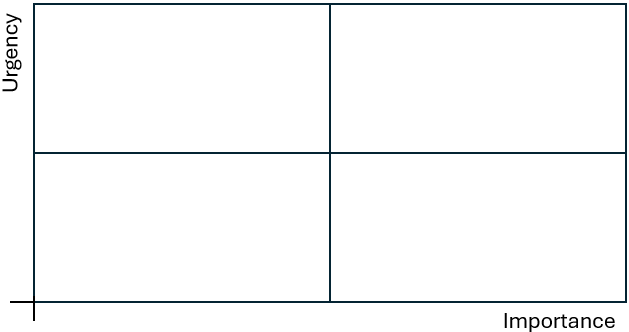
\includegraphics[width=.5\linewidth]{urgencyImportanceChart.png}

  You can plot your tasks on a chart like this and then decide to work on the most important \& urgent tasks first, then the most urgent, etc.
\end{figure}

\underline{Best Practices}

1. Goals alignment, breakdown to Tasks, Planning, Logging/Analysing, Observe/Reflect/Improve (the framework above)

2. Keep a “To-Do” List and a Schedule (with some free time to allow for flexibility/unexpected events)

3. Develop some habits that boost your efficiency (e.g., taking the first hour of the day to reply to all emails from the previous day)

4. Avoid procrastination and reward yourself for achieving goals. It’s always better to start a task…

5. Avoid destructions and interruptions. Focus!

6. Take breaks! (to refresh your mind)

7. Delegate. (Can save you a lot of time!)

8. Learn to say “No”. (Ensure scope is only as large as it needs to be)

9. Mentor colleagues to bring you problems accompanied with proposals for solutions. Not merely problems!

10. Prioritize (first things first) (e.g. quadrant of Urgent Vs Important tasks/activities) ("When everything is urgent, nothing is important")

11. Consult others on their practices and make sure you respect their time!

12. Manage your Energy!

\section{Meetings Management}

There exist various types of meetings, e.g. to share information, to resolve a problem, to make
decisions.

In most cases, there are a number of Questions and Best Practices that are applicable.

\underline{Before the Meeting}

\bulletPoint “To call or not to call”? (Do you actually need a meeting?)

\bulletPoint  An appropriately designed Agenda is a key success factor (should include sufficient time, appropriate venue, well
defined goals and concrete items with designated time) (Meetings should have predefined items to discuss)

\bulletPoint  Who to invite? (power to decide, have required info, have a role/interest in the topic, should be aware of
outcomes/facts to be presented, may be assigned actions)\\
people have a tendency to assign actions to people that are not in the
meeting (e.g., if they skipped it or weren't told about it), so you should
always attend if you suspect that you will be assigned an action, and react if
you disagree with the action

\bulletPoint  How many shall I invite? \\
(if you have to resolve a problem or make a decision, more than 8 participants may be an issue (they are not usually productive due to too much disagreement, too many people saying different things, lack of focus, etc.))\\
(If you are just sharing information, you could have 100s of people, it does not matter)

\bulletPoint  Organize and test the meeting venue conditions in advance! (lights, projector, paper, etc.)

\bulletPoint  Prepare yourself in advance (relevant documents/facts, communicate agenda and background material beforehand,
inform your boss or others who will not attend but are interested)

\bulletPoint  Decide on “How shall we decide”? (majority, unanimous, leader?) Which is better?

\underline{During the Meeting}

\bulletPoint Start at the time scheduled. Do not wait!\\
There is only one case in which you should wait - if a decision maker has not arrived yet in the meeting and they are the singular person who can make a decision for the meeting\\
Ask for permission to record the meeting

\bulletPoint If people do not know each other, allow time to introduce themselves

\bulletPoint The first action is to remind the topic, goals and the agenda items (and allow for possible reasonable adaptations)

\bulletPoint Discuss/decide any applicable rules (e.g. how to decide, timings, who will speak, decide on breaks in long meetings)

\bulletPoint Follow the agenda, do not allow irrelevant topics. Focus!\\
If something is useful, you can organize another meeting to discuss it. Do not let it take over the current one

\bulletPoint Facilitate/encourage participation and consensus, ask questions, be the “devils advocate”, exercise “Active Listening”, regularly
provide a synopsis of what has been discussed/decided.

\bulletPoint Build on positive aspects or items of agreement to continue.

\bulletPoint Do not permit interruptions or somebody dominating. Prevent/disallow interpersonal conflicts or disruptive behavior.

\bulletPoint Use the board to keep notes and highlight key points (but do not exaggerate)

\bulletPoint Keep track of time and progress to ensure the meeting is on-track. Try to finish on-time or ask permission if you wish to extend.

\bulletPoint Before the end, summarize what has been decided and make sure there are decision and action items/plan, with clear
responsibilities, schedules and review mechanisms!

\underline{After the Meeting}

\bulletPoint   Communicate appropriate Meeting Minutes (the notes from the meeting, meeting recording, etc.) in a timely manner.\\
Add "If amendments need to be made, please let me know"\\
Add "If I do not hear back from x date, then I will assume ... (everyone has agreed on what occurred)"

\bulletPoint   Reflect on your practices and aim to improve. If necessary, ask relevant participants on their views

\section{Conflict Management}

Conflict Definition: “a process, that begins when you \textit{perceive} that someone has frustrated or is
about to frustrate a major concern of yours”.

Two important elements:\\
\bulletPoint It is a process, not a state, i.e. it evolves! (not necessary in terms of actions, can be in term of feelings)\\
\bulletPoint It is perceptual, i.e. the parties involved “perceive”! (in different ways)\\
(disagreement does not equal conflict, but can lead to it)

3 main Categories;\\
\bulletPoint Goal-oriented conflicts – disagreements about results, performance criteria, objectives, priorities, etc.
Such conflicts often originate from multiple perceptions of the project which stem from vague goals which
trigger different individual interpretations. \\
\bulletPoint Administrative conflicts – arise through management hierarchy, structures and company philosophy. Such
conflicts are often centered on disagreements around authority/responsibility (e.g. project tasks,
decisions)\\
\bulletPoint Interpersonal conflict – due to personality differences, sources may include behavioural styles, egos,
ethics, personality traits, bias etc.

3 Schools of Thought: Traditional (conflict is negative), Behavioural, Interactionist (Conflict is a means for society making progress)

Numerous Sources of conflict, for example:\\
\bulletPoint Competition of scarce resources\\
\bulletPoint Organizational reward systems (e.g., bonuses)\\
\bulletPoint Uncertainty over lines of authority \\
\bulletPoint Departmental mindsets and agendas \\
\bulletPoint Violations of group or organizational norms (e.g., letting someone know you have delivered a piece of work or will do it late, etc.)\\
\bulletPoint Disagreements over goals and means to achieve them \\
\bulletPoint Faulty attributions\\
\bulletPoint Personal Fears and Biases\\
\bulletPoint Faulty Communication.\\
\bulletPoint ….

\underline{Main methods of Resolving Conflict}

1. Mediate\\
Directly and actively seek to find a solution. Options of “defusion”
(not finding the underlying cause of the conflict and simply making statements
that allow people to continue working together without necessarily resolving
the conflict) Vs
examining underlying causes. Requires working with both parties to come to a
common agreement.

2. Arbitrate\\
Impose a judgement after listening to both positions. Beware not to make
interpersonal judgement– put emphasis on facts and on the judgement itself.

3. Control\\
Not all conflicts should be quickly resolved. A pragmatic response may be to
wait for some time until parties cool down. Then intervene. (Let the situation
develop, observe it and then intervene at the right time)

4. Accept\\
Do nothing. Remember that sometimes by intervening, you may have a worse
result. Sometimes one may not know the full story (or history).

5. Eliminate\\
Remove conflicting party or parties from the project.

\underline{Best Practices}

1. Conflict is natural– it may even be an evidence of progress (but there is a limit).\\
consider the different leadership approaches

2. Different “resolution” approaches are appropriate in different situations.

3. No interference may be a good approach– its not about being “lazy”. In any case, carefully Plan the way
to intervene.

4. Learn to deal with your own conflicts and emotions constructively (in order to deal effectively with other
people conflicts).

5. Dealing with human emotions is usually more effective than rational argumentation.

6. Important to achieve that each party strives to experience “reality” using the other party’s “lenses” and
to focus on the other party’s emotions and concerns.

7. Encourage “Active Listening”.

8. 5-Why analysis. Beware of faulty assumptions and explore underlying motives. Accept and explore the
possibility that something that you (as PM) do (or do not do) may be the source of the conflict.

9. Better to strive for Collaborative “Win-Win” solutions

\chapter{Fundamentals of Project Quality Management}

Quality (Prince2 and ISO 9000): “The degree to which a set of inherent characteristics of a product,
service, process, person, organization, system or resource fulfils requirements.”

Quality Management (Prince2): “The coordinated activities to direct and control an organization
with regard to quality.”

Different Levels of Quality Management: Organizational Vs Project

At the organizational (corporate) level, quality management is concerned with establishing and
operating a framework of organizational processes and standards, e.g. ISO 20000 (ITIL-based)

At the project level, quality management involves\\
(i) the application of specific processes and verifying that these planned processes have been followed (typically according to the organizational processes) and\\
(ii) ensuring that that the produced products meet established quality criteria (quality specifications and measurements)

Quality Management Process Groups (IS0 21500) (what you do in a project);\\
1. Plan Quality (Planning)\\
2. Perform Quality Assurance (Implementing)\\
3. Perform Quality Control (Control Process group)

\section{Plan Quality}

"Specify how the project is going to be organized, in terms of quality, e.g.,
are we doing quality reviews?, what are the requirements of the end product?"

Output: Quality Plan

“The purpose of Plan quality is to determine the quality requirements and standards that will be applicable to
the project, the deliverables of the project and how the requirements and standards will be met based on the
project objectives.

This process includes the following:\\
\bulletPoint determining and agreeing with the project sponsor and other stakeholders as to the objectives and
relevant standards to be achieved;\\
\bulletPoint establishing the tools, procedures, techniques and resources necessary to achieve the relevant standards;\\
\bulletPoint determining methodologies, techniques and resources to implement the planned systematic quality
activities;\\
\bulletPoint developing the quality plan which includes type of reviews, responsibilities and participants in a timetable
in accordance with the project overall schedule;\\
\bulletPoint consolidating all quality information in the quality plan.

Due to the temporary nature of projects and their time constraints, most projects do not have the ability to
develop quality standards. Development and organizational acceptance of quality standards and product
quality parameters may be outside of the project boundaries.

This acceptance is normally the responsibility of
the performing organization and serves as input to this process. The quality plan should refer to or include the
quality policy as established by senior management.”

\section{Perform Quality Assurance}

"Review the deliverables and the projects"

“The purpose of Perform quality assurance is to review the deliverables and the project. It includes all
processes, tools, procedures, techniques and resources necessary to meet quality requirements.

This process includes the following:\\
\bulletPoint ensuring objectives and relevant standards to be achieved are communicated, understood, accepted and
adhered to by the appropriate project organization members;\\
\bulletPoint executing the quality plan as the project progresses;\\
\bulletPoint ensuring that the established tools, procedures, techniques and resources are being used.

Quality assurance audits \textbf{may be performed outside the project boundaries by other parts of the performing
  organization or by the customers}. Audits determine the performance of the quality \textbf{process}, quality \textbf{control}
and the \textbf{need for recommended actionor change requests}.”

In essence, “Quality assurance provides a check that the project’s direction and management are adequate for
the nature of the project and that it complies with relevant corporate or programme management standards
and policies.” (Prince2)

\underline{Quality Assurance Vs Project Assurance (Prince2)}

“Quality
assurance provides a check that the project’s direction and management are adequate for the
nature of the project and that it complies with relevant \textbf{corporate, programme management or customer
  standards and policies}. Quality assurance is therefore \textbf{independent} of the project.”\\
(An audit of processes and practices applied to reach the end product, e.g., instead of performing a stress
test, they will ask have you done a stress test?, when?, what are the results?, how did you interpret them?,
etc., did you make a risk register?, etc.)

What is found from this is called an audit finding.

“Project
assurance is the \textbf{project board’s (steering committee) responsibility to assure itself that the project is being conducted
  correctly}. The project board members each have a specific area of focus for project assurance, namely
business assurance for the executive, user assurance for the senior user(s) and supplier assurance for the
senior supplier(s). Project assurance is therefore \textbf{independent of the project manager but not independent of
  the project}.”

\newpage

\section{Perform Quality Control}

“The purpose of Perform quality control is to determine whether the established project objectives, quality
requirements and standards are being met and to identify causes of, and ways to eliminate, unsatisfactory
performance.

This process should be applied during the whole project life cycle and includes the following:\\
\bulletPoint monitoring the quality of the deliverables and processes is being met and detecting defects by using the
established tools, procedures and techniques;\\
\bulletPoint analysing possible causes of defects;\\
\bulletPoint determining the preventive actions and change requests;\\
\bulletPoint communicating the corrective actions and change requests to the appropriate project organization members.

Quality control may identify causes of poor process performance or product quality and may result in
recommendedactions or change requests, when necessary to eliminate non-conforming performance.

In essence (Prince2), “Quality control focuses on the operational techniques and activities used by those involved
in the project to:\\
\bulletPoint Fulfil the requirements for quality (for example, by quality inspections or testing)\\
\bulletPoint Identify ways of eliminating causes of unsatisfactory performance (for example, by introducing process
improvements as a result of lessons learned).”

\begin{figure}[H]
  \centering
  \includegraphics[width=\linewidth]{quality_reg.png}

  Quality Register (Prince2)\\
  “Summarize all the quality management activities that are planned or have taken place, and provides
  information for the end stage reports and end project report.”
\end{figure}

\newpage

\subsection{Software/IT Systems Testing Overview}

Quality aspect (what you are verifying): quality of the end product

Types;\\
\bulletPoint Performance/Stress Testing\\
\bulletPoint Security Testing\\
\bulletPoint Scalability and High-Availability Testing\\
\bulletPoint Disaster Recovery Testing\\
\bulletPoint….\\
Note that there are often difference in terminology to refer to
similar “things” with “some” differences (e.g. Integration Vs System
Vs Regression Vs Release Testing).

Who performs the testing is also a key factor

Automated testing saves a lot of effort but often you cannot avoid
Manual (typically tool assisted) testing

Test management tools organize the testing process (recording scenarios (steps),
plan testing (who, what, in what order, etc.), statistics, etc.)

\begin{figure}[H]
  \centering
  \includegraphics[width=.7\linewidth]{testingOverview.png}
\end{figure}

\newpage

\subsection{Software/IT Systems Testing Process}

\begin{figure}[H]
  \centering
  \includegraphics[width=\linewidth]{SoftwareIT Systems Testing Process.png}
\end{figure}

prioritize tests and ensure you have the relevant test data for each test

\subsection{Common Software Quality Attributes}

There is often a tension between customer/end user quality requirements (efficiency, reliability, etc.) and
developers quality requirements (maintainability, reusability, etc.)

Some quality requirements are difficult to specify in an unambiguous way

It is very difficult for any system to be optimized for all of these attributes. Therefore, the quality plan
should define the most important quality attributes.

The plan should also include a definition of the quality
assessment process, an agreed way of assessing/measuring whether desired quality attributes are present
in the product.

Attributes include;\\
\begin{minipage}[]{.3\linewidth}
  \bulletPoint Safety\\
  \bulletPoint Security\\
  \bulletPoint Reliability\\
  \bulletPoint Resilience\\
  \bulletPoint Robustness
\end{minipage}
\hfill
\begin{minipage}[]{.3\linewidth}
  \bulletPoint Understandability\\
  \bulletPoint Testability\\
  \bulletPoint Adaptability\\
  \bulletPoint Modularity\\
  \bulletPoint Complexity
\end{minipage}
\hfill
\begin{minipage}[]{.3\linewidth}
  \bulletPoint Portability\\
  \bulletPoint Usability\\
  \bulletPoint Reusability\\
  \bulletPoint Efficiency\\
  \bulletPoint Learnability
\end{minipage}

\newpage

\subsection{Quality Standards}

Definition (ISO): ”requirements, specifications, guidelines or characteristics that can be used consistently to
ensure that materials, products, processes and services are fit for their purpose.” Guidance Vs Requirements
standards.

Advantages of standards: encapsulation of best practice - avoids repetition of past mistakes, framework for
defining what quality means in a particular setting\\
i.e. that organization’s view of quality, they provide
continuity - new staff can understand the organisation by understanding the standards that are used.

ISO 9000 (principles) and ISO 9001 (requirements): General standards that can be used as a basis for
developing quality management systems.

Can be considered as a “framework” for developing organizational quality standards. It sets out general
quality principles, describes quality processes in general and lays out the organizational standards and
procedures that should be defined. These should be documented in an organizational quality manual.

In essence, ISO 9001 governs the implementation and maintenance of a quality management system,
ensures organizations’ processes are managed, documented, and continually improve. It is applicable to any
organization and industry (and may be “certified”).

\begin{figure}[H]
  \centering
  \includegraphics[width=\linewidth]{ISO 9001 Quality Standard.png}
\end{figure}

There are various levels of quality up to the organization
level

\newpage

\subsection{Continuous Process Improvement Process}

Acrucial requirement/characteristic/attribute. Part of overall Total Quality Management (TQM).

There is no ‘ideal’ or ‘standard’ process that is applicable in all organizations or for all software/IT
products/projects of a particular type.

It is rarely successful in introducing process improvements
if you simply attempt to change the process to one that is used elsewhere. One should consider
the local environment and culture and how this may be affected by process change proposals.

Each company typically develops its own process depending on its size, the background and skills
of its staff, the type of software/IT system being developed, customer and market requirements,
and the company culture.

In continuous process improvement one has to consider what aspects of the process to improve
(e.g. product quality, process itself (e.g. development time)?

There are several approaches in Process Improvement. Common Steps:\\
1. Identification of goals \\
2. Analysis of the present situation \\
3. Development of an approach/solution \\
4. Construction of a plan \\
5. Execution of the plan  \\
6. Measurement of results

\begin{figure}[H]
  \centering
  \includegraphics[width=\linewidth]{pdca.png}
\end{figure}

Plan; identify the problem \& analyze it\\
Do; find the solution or a potential solution\\
Check; evaluate the results \& see if the solution works\\
Act; determine the next steps

\end{document}
\end{article}